\chapter[Desenvolvimento do Projeto]{Desenvolvimento do Projeto}

O capítulo apresenta o projeto realizado nessa dissertação, contendo a explicação do que foi desenvolvido, os circuitos esquemáticos, e os parâmetros dos componentes. Alguns circuitos não foram incluídos neste capítulo e são apresentados de maneira implícita, devido à sua simplicidade, flexibilidade de implementação em replicações do trabalho, e o autor também entender que os mesmos já sejam de amplo conhecimento na área. No \autoref{blocosadicionais} é possível verificar mais sobre esses blocos e como foram desenvolvidos, caso o leitor sinta a necessidade de entender a sua implementação.

\newcommand{\NomeBloco}{NULL}
\newcommand{\NomeBlocoNoIt}{NULL}
\newcommand{\NomeBlocoNoUnderline}{NULL}
\newcommand{\NomePTab}{tab_\NomeBlocoNoUnderline}
\newcommand{\NomeSTab}{tab_\NomeBlocoNoUnderline2}
\newcommand{\NomePFig}{fig_\NomeBlocoNoUnderline}
\newcommand{\NomeSFig}{fig_\NomeBlocoNoUnderline2}
\newcommand{\NomeTTab}{tab_\NomeBlocoNoUnderline3}
\newcommand{\NomeQTab}{tab_\NomeBlocoNoUnderline4}

Um circuito integrado foi desenvolvido para avaliar cinco dispositivos APS's, referenciado na se{\c c}\~ao \ref{section:APS} deste documento, e dois TIA's, em refer\^encia \`a se{\c c}\~ao \ref{section:TIA}. O projeto \'e representado em alto n\'ivel na \autoref{fig_circcompleto}. Todos os sinais aqui apresentados na figura, e tamb\'em em todas figuras \'a seguir, seguem o a padr\~o descrito na se{\c c}\~ao \ref{section:padrao_sinais} deste trabalho.

\begin{figure}[htb]
	\caption{\label{fig_circcompleto}Circuito projetado}
	\begin{center}
	    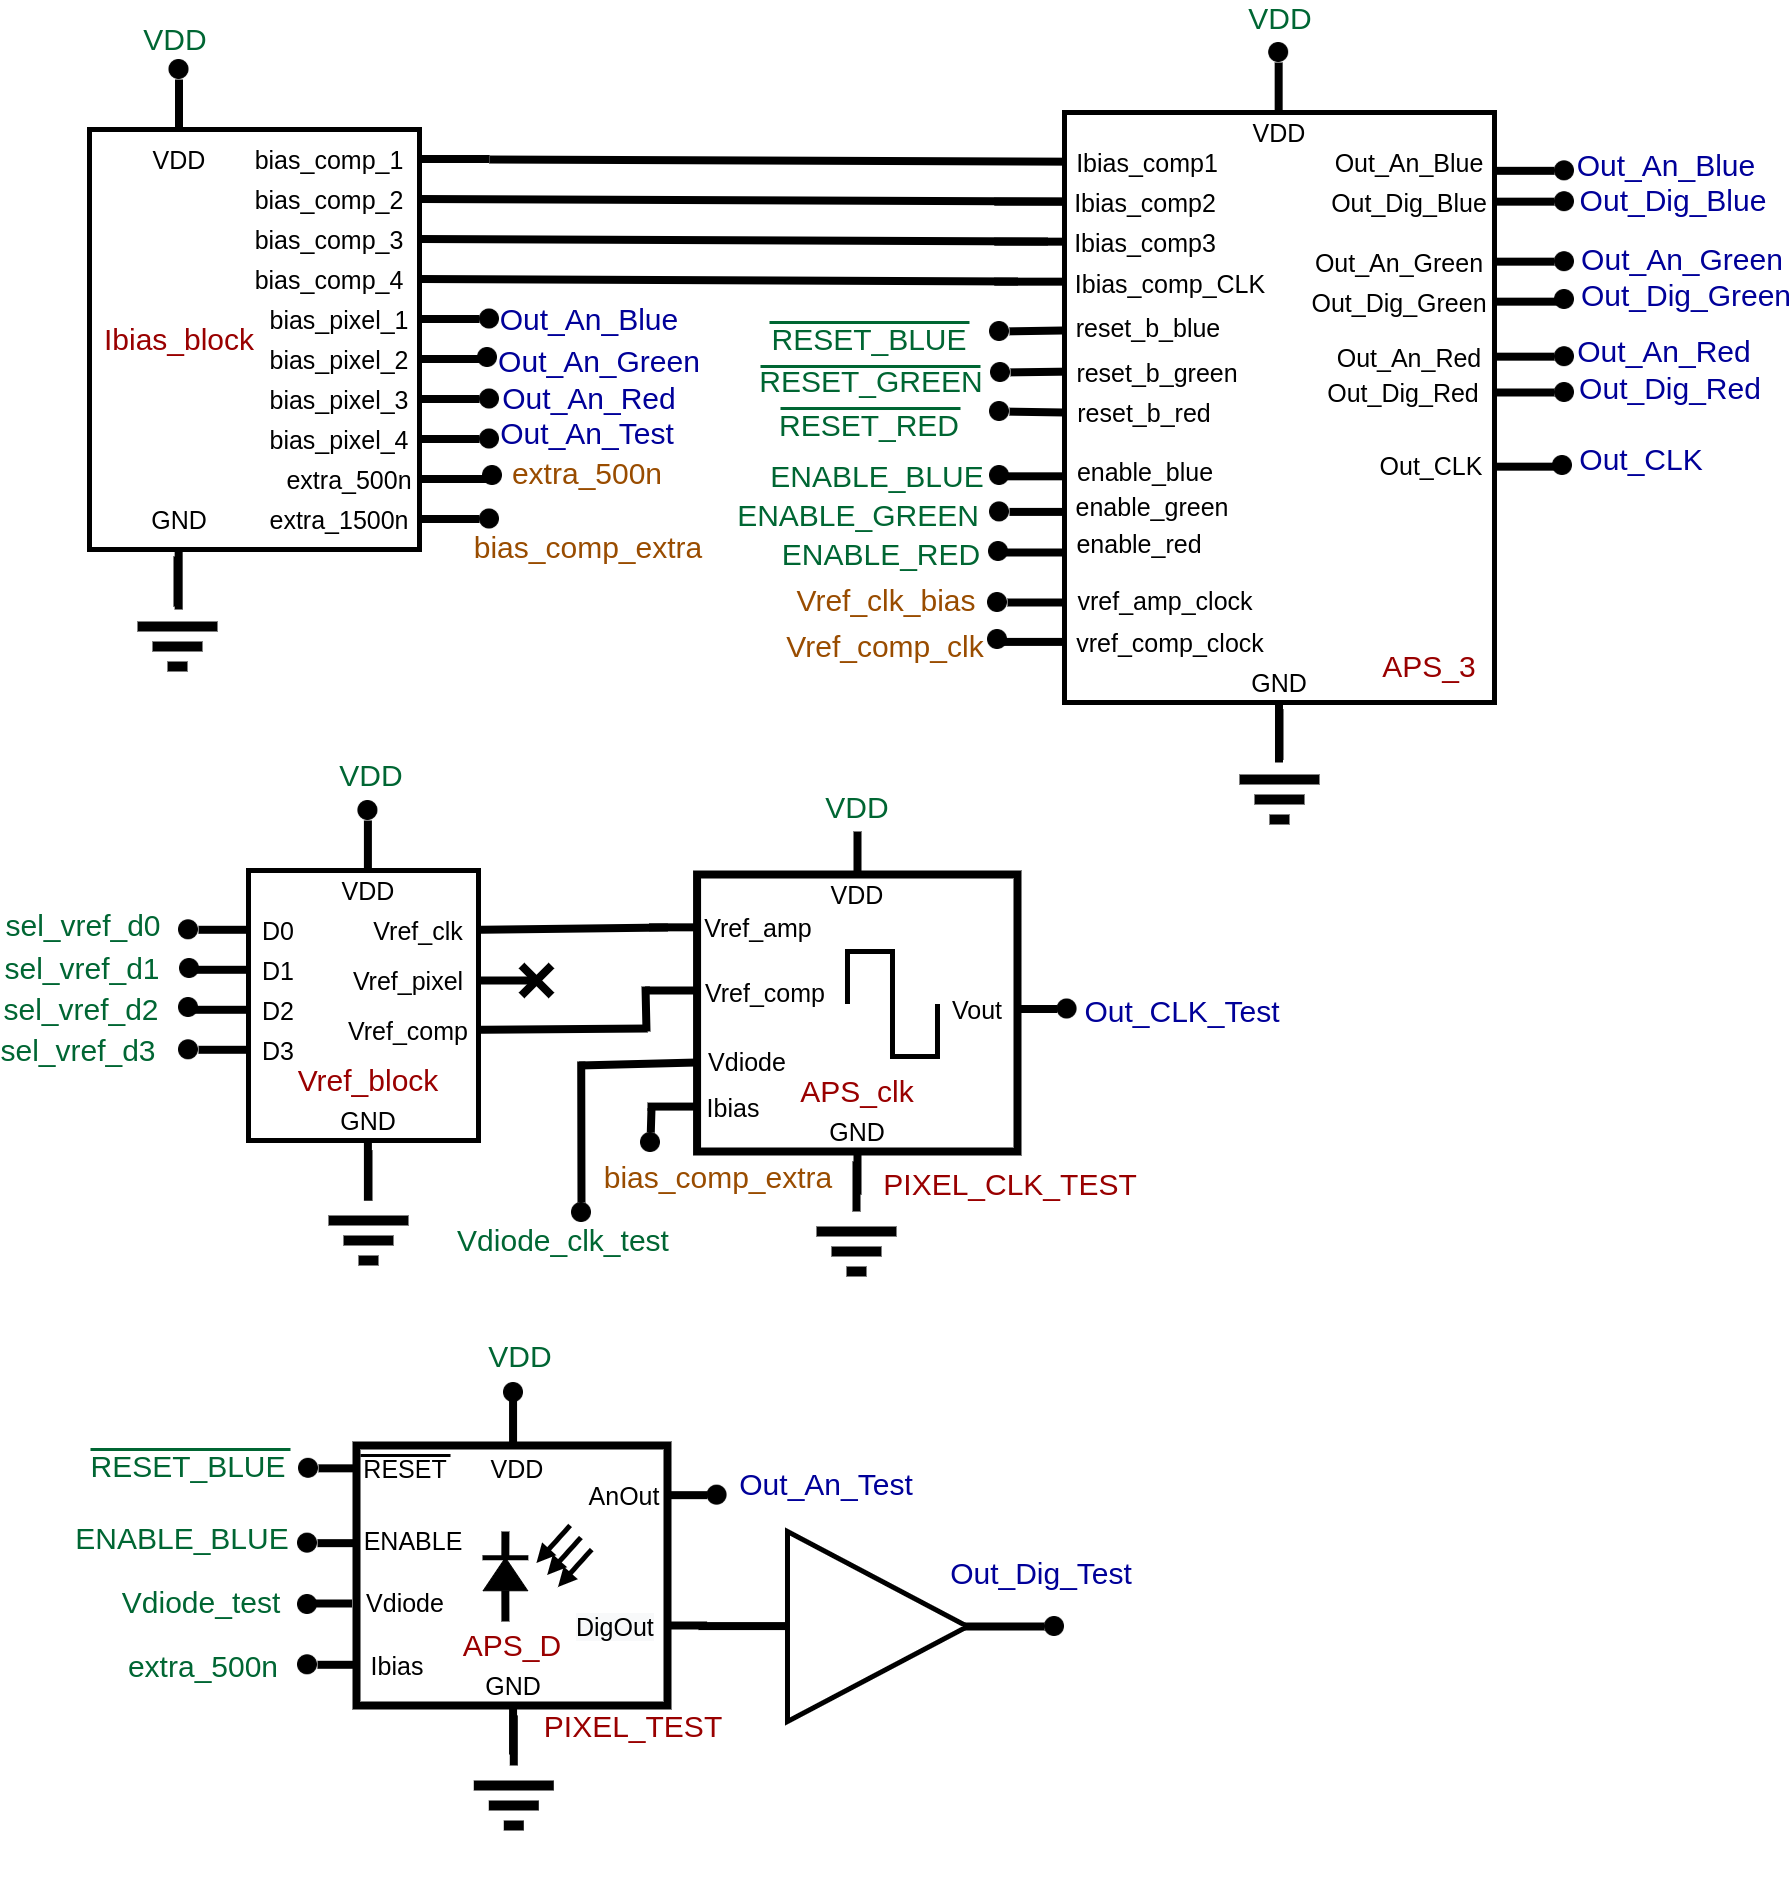
\includegraphics[width=\textwidth]{Circuitos/Complete_Circuit.png}
	\end{center}
	\legend{Fonte: Produzido pelo autor}
\end{figure}

O circuito tem a finalidade de processar a informa{\c c}\~ao advinda de tr\^es APS's, constru\'idos de maneira id\^entica em n\'ivel de layout, com a finalidade de abstrair informa{\c c}\~oes de cores advindas de uma fonte luminosa, dos quais podem ser Azul, Verde ou Vermelha. Para que as cores fossem devidamente separadas entre cada APS, filtros luminosos externo, por meio de uma pel\'icula colorida, s\~ao adicionados sob cada APS respons\'avel por processar uma cor equivalente \`a de sua pel\'icula.

Um sinal luminoso de cor branca tamb\'em \'e utilizado no sistema de forma a ser a refer\^encia de rel\'ogio de todos APS's descritos. Esse sinal \'e processado utilizando-se um $TIA$, do qual \'e gerado um sinal el\'etrico equivalente \'a informa{\c c}\~ao luminosa.

A tecnologia de fabrica{\c c}\~ao utilizada para o desenvolvimento de todos blocos foi a \emph{CMOS 180nm da TSMC}. O software utilizado para o projeto do dispositivo foi o \emph{Virtuoso}, desenvolvido pela \emph{Cadence}.

O circuito representado na \autoref{fig_circcompleto} \'e composto por 2 blocos principais, que permitem o processamento advindos da fonte luminosa, al\'em de um circuito \emph{APS} e um \emph{TIA} extra. A descri{\c c}\~ao dos bloco s\~ao:

\begin{itemize}
    \item \emph{ibias\_block}: Tem a fun{\c c}\~ao de gerar todas fontes de corrente utilizadas em todos os blocos do circuito, quando necess\'ario.
    
    \item \emph{4\_APS}: Implementa os tr\^es circuitos APS descritos, al\'em do circuito \emph{TIA}. A sa\'ida de cada bloco passa por um comparador de forma a digitalizar o dado, como ser\'a melhor explicitado na se{\c c}\~ao \autoref{Bloco4APS}.
    
    \item \emph{Vref\_block} e \emph{PIXEL\_CLK\_TEST}: Estes blocos realizam a implementa{\c c}\~ao de um TIA, por\'em com a adi{\c c}\~ao de um pino extra que possibilita a simula{\c c}\~ao de uma corrente fotogerada sem necessitar de uma fonte luminosa. Estes blocos ser\~ao melhor explicados na se{\c c}\~ao \autoref{BlocoTIA}. 
    
    \item \emph{Vref\_block} e \emph{PIXEL\_TEST}: Este blocos realizam a implementa{\c c}\~ao de um APS, por\'em com a adi{\c c}\~ao de um pino extra que possibilita a simula{\c c}\~ao de uma corrente fotogerada sem necessitar de uma fonte luminosa. Estes blocos ser\~ao melhor explicados na se{\c c}\~ao \autoref{BlocoAPS}.
    
\end{itemize}

A \autoref{tab_circcomp} mostra a rela{\c c}\~ao de sinais de entrada e sa\'ida presentes no circuito, para o processamento dos p\'ixels de cor. A \autoref{tab_circcomp2} mostra a rela{\c c}\~ao de sinais de entrada e sa\'ida presentes no circuito para o processamento dos blocos de teste.

\begin{table}[htb]
\IBGEtab{%
  \caption{Descri{\c c}\~ao dos sinais de entrada e sa\'ida do circuito projetado para as cores azul, verde e vermelha}%
  \label{tab_circcomp}
}{%
  \begin{tabular}{ccll}
  \toprule
   Sinal & Tipo & Descri{\c c}\~ao & Observa{\c c}\~ao \\
  \midrule \midrule
   RESET\_BLUE & Entrada & Sinal de \emph{RESET} no APS para cor azul & Ativo em n\'ivel baixo \\
  \midrule
   RESET\_GREEN & Entrada & Sinal de \emph{RESET} no APS para cor verde & Ativo em n\'ivel baixo \\
  \midrule
   RESET\_RED & Entrada & Sinal de \emph{RESET} no APS para cor vermelha & Ativo em n\'ivel baixo \\
  \midrule
   ENABLE\_BLUE & Entrada & Sinal de \emph{ENABLE} no APS para cor azul & Ativo em n\'ivel alto \\
  \midrule
   ENABLE\_GREEN & Entrada & Sinal de \emph{ENABLE} no APS para cor verde & Ativo em n\'ivel alto \\
  \midrule
   ENABLE\_RED & Entrada & Sinal de \emph{ENABLE} no APS para cor vermelha & Ativo em n\'ivel alto \\
  \midrule
   Out\_An\_Blue & Sa\'ida & Sinal anal\'ogico para cor azul \\
  \midrule
   Out\_Dig\_Blue & Sa\'ida & Sinal digital para cor azul \\
  \midrule
   Out\_An\_Green & Sa\'ida & Sinal anal\'ogico para cor verde \\
  \midrule
   Out\_Dig\_Green & Sa\'ida & Sinal digital para cor verde \\
  \midrule
   Out\_An\_Red & Sa\'ida & Sinal anal\'ogico para cor vermelha \\
  \midrule
   Out\_Dig\_Red & Sa\'ida & Sinal digital para cor vermelha \\
  \bottomrule
\end{tabular}%
}{%
  \fonte{Produzido pelo autor.}
}
\end{table}

\begin{table}[htb]
\IBGEtab{%
  \caption{Descri{\c c}\~ao dos sinais de entrada e sa\'ida do circuito projetado para os blocos de teste}%
  \label{tab_circcomp2}
}{%
  \begin{tabular}{cccc}
  \toprule
   Sinal & Tipo & Descri{\c c}\~ao & Observa{\c c}\~ao \\
  \bottomrule
\end{tabular}%
}{%
  \fonte{Produzido pelo autor.}
}
\end{table}
\section{Espelhos de Corrente}

Espelhos de Corrente foram necess\'arios para o desenvolvimento de diversos blocos contidos no projeto, e ser\~ao especificados nas subse{\c c}\~oes \` seguinte. Uma explica{\c c}\~ao geral sobre o funcionamento e desenvolvimento de espelhos de corrente pode ser visto na \autoref{anexoespelhos}.

\renewcommand{\NomeBloco}{ibias\_generator}
\renewcommand{\NomeBlocoNoUnderline}{ibiasgenerator}
\renewcommand{\NomePTab}{tab_\NomeBlocoNoUnderline}
\renewcommand{\NomeSTab}{tab_\NomeBlocoNoUnderline2}
\renewcommand{\NomePFig}{fig_\NomeBlocoNoUnderline}
\renewcommand{\NomeSFig}{fig_\NomeBlocoNoUnderline2}
\renewcommand{\NomeTTab}{tab_\NomeBlocoNoUnderline3}
\renewcommand{\NomeQTab}{tab_\NomeBlocoNoUnderline4}

\subsection{ibias\_generator}
 
O bloco \NomeBloco{}\footnote{Circuito desenvolvido pelo aluno \textit{Daniel Carvalho Lott}, do curso de bacharelado em Engenharia Elétrica da UFMG, no ano de 2020} \'e um espelho de corrente que apresenta uma sa\'ida de 50 $\mu$A. O bloco apresenta as definições de sinais de entrada e sa\'ida referidos na \autoref{\NomeSTab}.

\begin{table}[htbp]
\caption{Sinais do bloco \NomeBloco}
\label{\NomeSTab}
\centering
\begin{tabular}{ccl}

    \toprule
    Sinal & Tipo    & Descrição        \\
    \midrule \midrule
    ibias\_1   & Saída   & Fonte de Corrente de 50 $\mu$A \\
    \bottomrule
\end{tabular}
\legend{Fonte: Produzido pelo autor}
\end{table}

O circuito projetado para o bloco \'e demonstrado na \autoref{\NomePFig}.

\begin{figure}[htb]
 \centering
    \centering
    \caption{Circuito CMOS projetado para o bloco \NomeBloco} 
    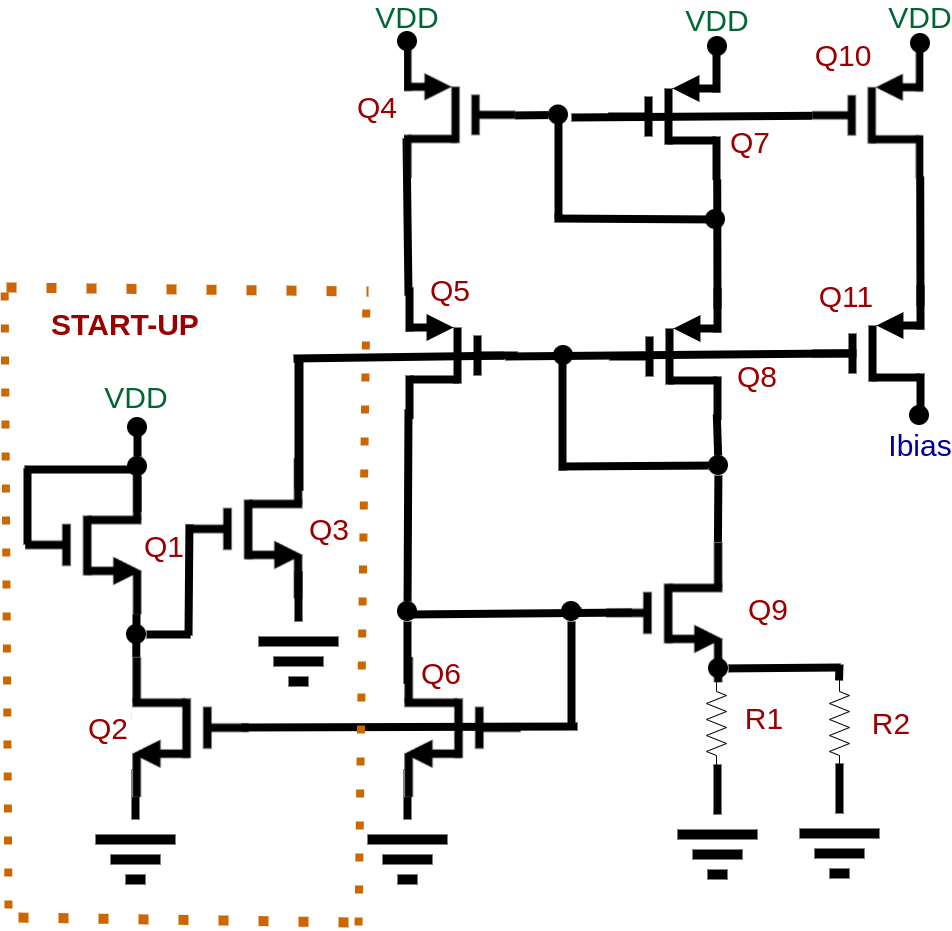
\includegraphics[scale=0.3]{Circuitos/Ibias_generator.png}
    \legend{Fonte: Produzido pelo autor}
    \label{\NomePFig}
\end{figure}

\begin{figure}[htb]
 \centering
    \centering
    \caption{Representação em bloco do \NomeBloco} \label{\NomeSFig}
    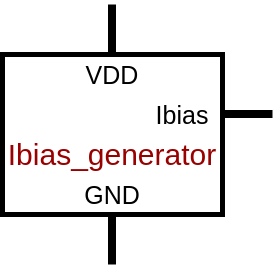
\includegraphics[scale=0.3]{Circuitos/ibias_generator_block.png}
    \legend{Fonte: Produzido pelo autor}
\end{figure}

Os transistores utilizados no bloco apresentam os par\^ametros mostrados na \autoref{\NomeTTab}.

\begin{table}[htbp]
\caption{Transistores do Bloco \NomeBloco}
\label{\NomeTTab}
\centering
\begin{tabular}{ccccc}
\toprule
Transistor & W ($\mu$m)  & L ($\mu$m)           & M (n° dispositivos) & S (n° dispositivos)\\
\midrule \midrule
Q1 & 0,3 & 19,995 & 1 & 3\\
\midrule
Q2 & 25 & 0,5 & 2 & 1\\
\midrule
Q3 & 30 & 0,5 & 1 & 1\\
\midrule
Q4, Q7 e Q10 & 35 & 4 & 2 & 1\\
\midrule
Q5, Q8 e Q11 & 25 & 2,5 & 2 & 1\\
\midrule
Q6 & 20 & 4 & 2 & 1\\
\midrule
Q9 & 20 & 4 & 4 & 1\\
\midrule
Q10 & 25 & 2,5 & 2 & 1\\
\midrule
Q11 & 25 & 2,5 & 2 & 1\\
\bottomrule
\end{tabular}
\legend{Fonte: Produzido pelo autor}
\end{table}

O resistor utilizado no bloco apresenta os par\^ametros mostrados na \autoref{\NomeQTab}.

\begin{table}[htbp]
\caption{Resistor do bloco \NomeBloco}
\label{\NomeQTab}
\centering
\begin{tabular}{ccccc}
\toprule
Resistor & W ($\mu$m)  & L ($\mu$m) & M (n° dispositivos) & Resist\^encia (k$\Omega$)\\
\midrule \midrule
R & 8 & 29,98 & 2 & 0,569025\\
\bottomrule
\end{tabular}
\legend{Fonte: Produzido pelo autor}
\end{table}

Os transistores \textit{Q6} e \textit{Q9}, juntos aos resistores \textit{R1} e \textit{R2}, t\^em a finalidade de funcionarem como um dreno de corrente referenciados pelos resistores. Os transistores \textit{Q4} e \textit{Q7} t\^em a finalidade de funcionarem como uma fonte de corrente, referenciados pelo dreno de corrente j\'a mencionado. O transistor \textit{Q10} \'e o braço do espelho de corrente do qual fornece a corrente de sa\'ida.

Os transistores \textit{Q5}, \textit{Q8} e \textit{Q11} se apresentam na configuração \textit{Cascode}, que tem o intuito de tornar o espelho de corrente de resposta mais linear, aumentar sua banda e ainda aumentar as suas resist\^encias de entrada e sa\'ida.

Os transistores \textit{Q1}, \textit{Q2} e \textit{Q3} t\^em a função de inicializar o circuito no ponto de operação adequado, j\'a que o circuito tamb\'em apresenta estabilidade quando fornecendo 0 A, sendo necess\'ario evitar essa situação.

\renewcommand{\NomeBloco}{\textit{iref\_generator}}
\renewcommand{\NomeBlocoNoUnderline}{irefgenerator}
\renewcommand{\NomePTab}{tab_\NomeBlocoNoUnderline}
\renewcommand{\NomeSTab}{tab_\NomeBlocoNoUnderline2}
\renewcommand{\NomePFig}{fig_\NomeBlocoNoUnderline}
\renewcommand{\NomeSFig}{fig_\NomeBlocoNoUnderline2}
\renewcommand{\NomeTTab}{tab_\NomeBlocoNoUnderline3}
\renewcommand{\NomeQTab}{tab_\NomeBlocoNoUnderline4}

\subsection{iref\_generator}

O bloco \NomeBloco{}\footnote{Circuito desenvolvido por \textit{Dalton Martini Colombo}, orientador do trabalho aqui apresentado} \'e um espelho de corrente que apresenta algumas sa\'idas como fonte e outras em dreno de corrente. O bloco apresenta as definições de sa\'ida referidos na \autoref{\NomeSTab}.

\begin{table}[!h]
\caption{Sinais do bloco \NomeBloco}
\label{\NomeSTab}
\centering
\begin{tabular}{ccl}

    \toprule
    Sinal & Tipo    & Descrição        \\
    \midrule \midrule
    iref1\_src   & Saída   & Fonte de Corrente de 0.5 $\mu$A \\
    \midrule
    iref2\_src   & Saída   & Fonte de Corrente de 0.5 $\mu$A \\
    \midrule
    iout\_test   & Saída   & Fonte de Corrente de 1.5 $\mu$A \\
    \midrule
    iref1\_sink   & Saída   & Dreno de Corrente de 0.5 $\mu$A \\
    \midrule
    iref2\_sink   & Saída   & Dreno de Corrente de 0.5 $\mu$A \\
    \bottomrule
\end{tabular}
\legend{Fonte: Produzido pelo autor}
\end{table}

O circuito projetado para o bloco \'e demonstrado na \autoref{\NomePFig}.

\begin{figure}[htb]
 \centering
    \centering
    \caption{Circuito CMOS projetado para o bloco \NomeBloco} 
    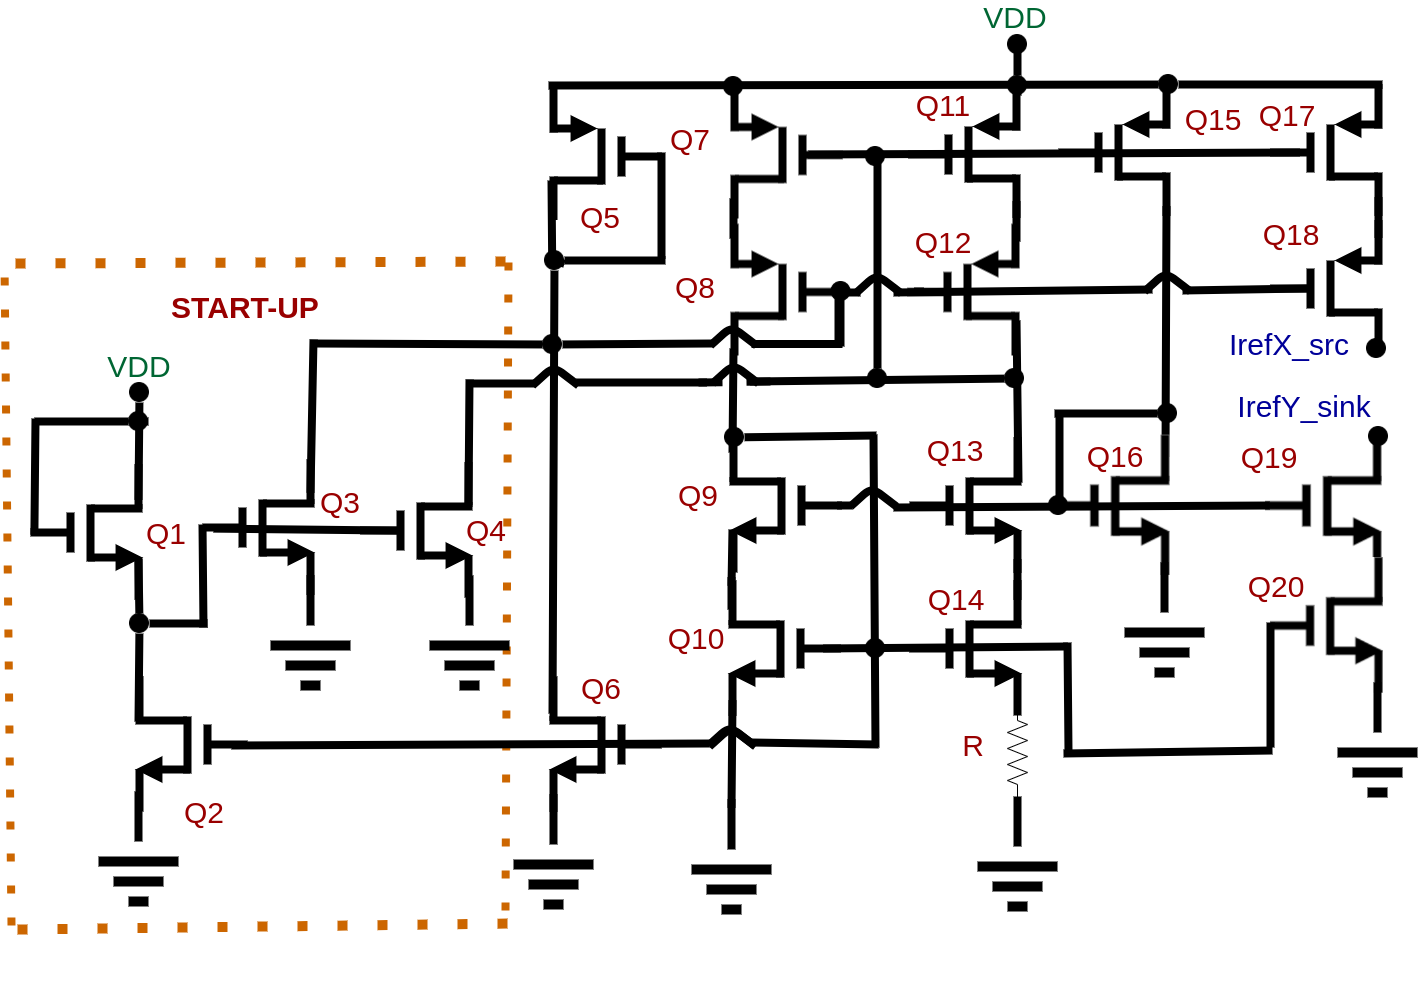
\includegraphics[scale=0.3]{Circuitos/iref_generator.png}
    \legend{Fonte: Produzido pelo autor}
    \nota{Nem todos transistores são representados na imagem. \emph{Q17}, \emph{Q18}, \emph{Q19} e \emph{Q20} são transistores replicados para cada sa\'ida \emph{IrefX\_src} e \emph{IrefY\_sink}, onde \emph{X} e \emph{Y} são os identificadores de cada sa\'ida}
    \label{\NomePFig}
\end{figure}

\begin{figure}[htb]
 \centering
    \centering
    \caption{\label{\NomeSFig}Representação em bloco do \NomeBloco}
    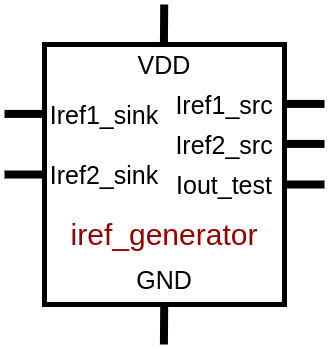
\includegraphics[scale=0.3]{Circuitos/iref_generator_block.png}
    \legend{Fonte: Produzido pelo autor}
\end{figure}

Os transistores utilizados no bloco apresentam os par\^ametros mostrados na \autoref{\NomeTTab}.

\begin{table}[!h]
\caption{Transistores do Bloco \NomeBloco}
\label{\NomeTTab}
\centering
\begin{tabular}{ccccc}
\toprule
Transistor & W ($\mu$m)  & L ($\mu$m)  & M (n° dispositivos) & S (n° dispositivos)\\
\midrule \midrule

\midrule
Q1                                   & 0,3    & 19,995 & 1                   & 3                   \\
\midrule
Q2                                   & 35     & 0,18   & 2                   & 1                   \\
\midrule
Q3 e Q4                              & 15     & 0,18   & 1                   & 1                   \\
\midrule
Q5                                   & 10     & 15     & 1                   & 6                   \\
\midrule
\begin{tabular}[c]{@{}c@{}}Q6, Q9, Q10,\\ Q13, Q19 e Q20\end{tabular}          & 4      & 19,995 & 1                   & 2                   \\
\midrule
\begin{tabular}[c]{@{}c@{}}Q7, Q8, Q11, Q12,\\ Q15, Q17a¹ e Q18a¹\end{tabular} & 10     & 15   & 2                   & 1                   \\
\midrule
Q14                                  & 4      & 19,995 & 10                  & 1                   \\
\midrule
Q16                                  & 4      & 19,995 & 1                   & 6 \\
\midrule
Q17b² e Q18b²                                                                  & 10     & 15     & 6                   & 1                  \\
\bottomrule
\end{tabular}
\legend{Fonte: Produzido pelo autor}
\legend{¹ Q17a e Q18a são os transistores referentes \`as sa\'idas iref1\_src e iref2\_src\\
² Q17b e Q18b são os transistores referentes \`a sa\'ida iout\_test}
\end{table}

O resistor \emph{R} utilizado no bloco apresenta os par\^ametros mostrado na \autoref{\NomeQTab}.

\begin{table}[!h]
\caption{Resistores do bloco \NomeBloco}
\label{\NomeQTab}
\centering
\begin{tabular}{cccc}
\toprule
Resistor & W ($\mu$m)  & L ($\mu$m) & Resist\^encia (k$\Omega$)\\
\midrule \midrule
R & 3 & 404,4 & 141,996\\
\bottomrule
\end{tabular}
\legend{Fonte: Produzido pelo autor}
\end{table}

Os transistores \emph{Q6} e \emph{Q9}, juntos aos resistores \emph{R1} e \emph{R2}, t\^em a finalidade de funcionarem como um dreno de corrente referenciados pelos resistores. Os transistores \emph{Q4} e \emph{Q7} t\^em a finalidade de funcionarem como uma fonte de corrente, referenciados pelo dreno de corrente j\'a mencionado. O transistor \emph{Q10} \'e o braço do espelho de corrente do qual fornece a corrente de sa\'ida.

Os transistores \emph{Q5}, \emph{Q8} e \emph{Q11} se apresentam na configuração \emph{Cascode}, que tem o intuito de tornar o espelho de corrente de resposta mais linear, aumentar sua banda e ainda aumentar as suas resist\^encias de entrada e sa\'ida.

Os transistores \emph{Q1}, \emph{Q2} e \emph{Q3} t\^em a função de inicializarem o circuito no ponto de operação adequado, j\'a que o circuito tamb\'em apresenta estabilidade quando fornecendo 0 A, sendo necess\'ario evitar essa situação.

\renewcommand{\NomeBloco}{current\_mirror\_nmos}
\renewcommand{\NomeBlocoNoUnderline}{curmirnmosb}
\renewcommand{\NomePTab}{tab_\NomeBlocoNoUnderline}
\renewcommand{\NomeSTab}{tab_\NomeBlocoNoUnderline2}
\renewcommand{\NomePFig}{fig_\NomeBlocoNoUnderline}
\renewcommand{\NomeSFig}{fig_\NomeBlocoNoUnderline2}
\renewcommand{\NomeTTab}{tab_\NomeBlocoNoUnderline3}
\renewcommand{\NomeQTab}{tab_\NomeBlocoNoUnderline4}

\subsubsection{\NomeBloco}

O bloco \NomeBloco{} cont\'em alguns bra{\c c}os utilizados como dreno de corrente para outras partes do circuito, sendo todos valores iguais \'a corrente de refer\^encia. O bloco apresenta as defini{\c c}\~oes de sinais de entrada e sa\'ida referidos na \autoref{\NomeSTab}.

\begin{table}[htbp]
\caption{Sinais do bloco \NomeBloco}
\label{\NomeSTab}
\centering
\begin{tabular}{ccl}

    \toprule
    Sinal & Tipo    & Descri{\c c}\~ao        \\
    \midrule \midrule
    Iref\_bias   & Entrada   &  Corrente de refer\^encia para os bra{\c c}os \\
    \midrule
    Iref\_A   & Saída   &  Bra{\c c}o 1 \\
    \midrule
    Iref\_B   & Saída   &  Bra{\c c}o 2 \\
    \midrule
    Iref\_C   & Saída   &  Bra{\c c}o 3 \\
    \midrule
    Iref\_D   & Saída   &  Bra{\c c}o 4 \\
    \midrule
    Iref\_E   & Saída   &  Bra{\c c}o 5 \\
    \bottomrule
\end{tabular}
\legend{Fonte: Produzido pelo autor}
\end{table}

O circuito projetado para o bloco \'e demonstrado na \autoref{\NomePFig}.

\begin{figure}[htb]
 \centering
    \centering
    \caption{Circuito CMOS projetado para o bloco \NomeBloco} 
    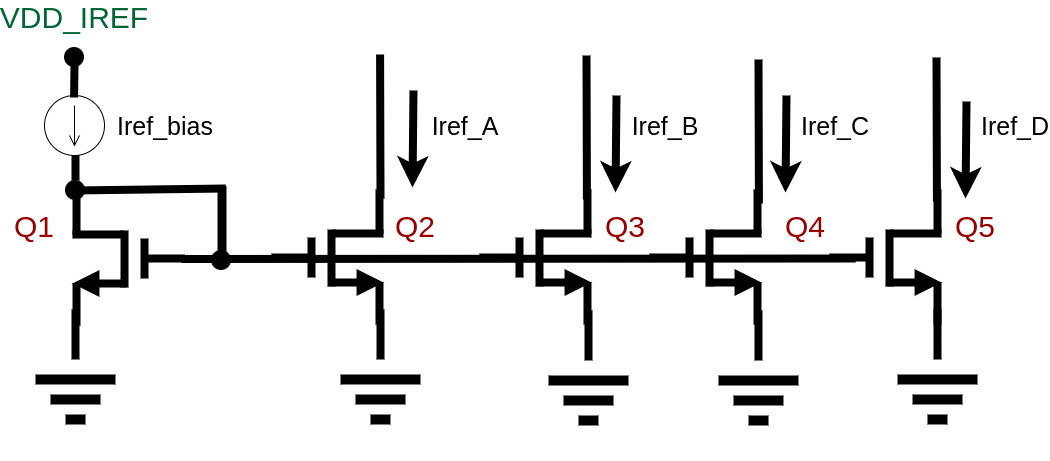
\includegraphics[scale=0.3]{Circuitos/current_mirror.png}
    \legend{Fonte: Produzido pelo autor}
    \label{\NomePFig}
\end{figure}

\begin{figure}[htb]
 \centering
    \centering
    \caption{Representa{\c c}\~ao em bloco do \NomeBloco} \label{\NomeSFig}
    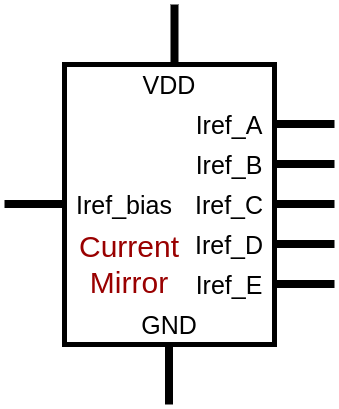
\includegraphics[scale=0.3]{Circuitos/current_mirror_block.png}
    \legend{Fonte: Produzido pelo autor}
\end{figure}

Os transistores utilizados no bloco \NomeBloco{} apresentam os par\^ametros mostrados na \autoref{\NomeTTab}.

\begin{table}[htbp]
\caption{Transistores do Bloco \NomeBloco}
\label{\NomeTTab}
\centering
\begin{tabular}{ccccc}
\toprule
Transistor & W ($\mu$m)  & L ($\mu$m)           & M (n° dispositivos) & S (n° dispositivos)\\
\midrule \midrule
\begin{tabular}[c]{@{}c@{}}Q1, Q2, Q3,\\
Q4, Q5 e Q6\end{tabular} & 5 & 6 & 2 & 1\\
\bottomrule
\end{tabular}
\legend{Fonte: Produzido pelo autor}
\end{table}

\renewcommand{\NomeBloco}{APS\_digitalized}
\renewcommand{\NomeBlocoNoUnderline}{apsdigitalized}
\renewcommand{\NomePTab}{tab_\NomeBlocoNoUnderline}
\renewcommand{\NomeSTab}{tab_\NomeBlocoNoUnderline2}
\renewcommand{\NomePFig}{fig_\NomeBlocoNoUnderline}
\renewcommand{\NomeSFig}{fig_\NomeBlocoNoUnderline2}
\renewcommand{\NomeTTab}{tab_\NomeBlocoNoUnderline3}
\renewcommand{\NomeQTab}{tab_\NomeBlocoNoUnderline4}

\section{\NomeBloco}

O \emph{APS\_digitalized} \'e o circuito respons\'avel por digitalizar o sinal gerado pelo APS descrito na \autoref{section:APS}. O bloco apresenta as defini{\c c}\~oes de sinais de entrada e sa\'ida referidos na \autoref{\NomeSTab}.

\begin{table}[htbp]
\caption{Sinais do bloco \NomeBloco}
\label{\NomeSTab}
\centering
\begin{tabular}{ccll}

    \toprule
    Sinal & Tipo    & Descri{\c c}\~ao & Observa{\c c}\~ao        \\
    \midrule \midrule
    RESET   & Entrada   & Sinal de RESET no APS & Ativo em nível baixo\\
    \midrule
    ENABLE   & Entrada   & Sinal de ENABLE no APS & Ativo em nível alto\\
    \midrule
    Vref   & Entrada   & Tens\~ao de refer\^encia utilizada pelo comparador \\
    \midrule
    Ibias   & Entrada   & Corrente de polariza{\c c}\~ao do comparador \\
    \midrule
    AnOut   & Saída   & Sinal anal\'ogico produzido pelo APS \\
    \midrule
    DigOut   & Saída   & Sinal digital produzido pelo Comparador \\
    \bottomrule
\end{tabular}
\legend{Fonte: Produzido pelo autor}
\end{table}

O circuito projetado para o bloco \'e demonstrado na \autoref{\NomePFig}.

\begin{figure}[htb]
 \label{\NomePFig}
 \centering
    \centering
    \caption{Circuito CMOS projetado para o bloco \NomeBloco} 
    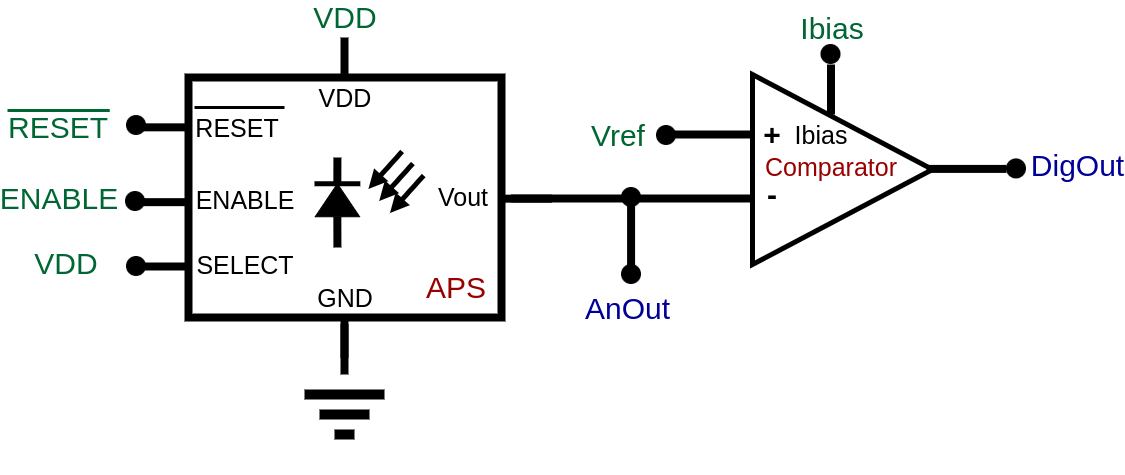
\includegraphics[scale=0.4]{Circuitos/APS_digitalized.png}
    \legend{Fonte: Produzido pelo autor}
\end{figure}

\begin{figure}[htb]
 \centering
    \centering
    \caption{Representa{\c c}\~ao em bloco do \NomeBloco} \label{\NomeSFig}
    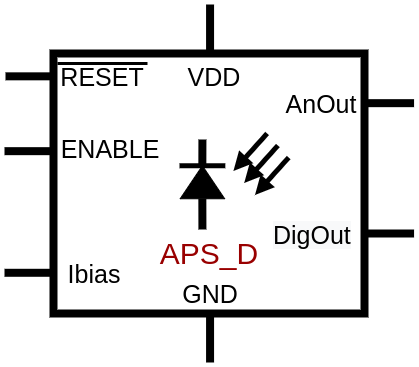
\includegraphics[scale=0.5]{Circuitos/APS_digitalized_block.png}
    \legend{Fonte: Produzido pelo autor}
\end{figure}

A sa\'ida digital do bloco funciona realizando uma compara{c c}\~ao entre uma tens\~ao de refer\^encia chamada de \emph{Vref} e a sa\'ida anal\'ogica do APS, chamada de \emph{AnOut}. Quando o valor de \emph{Vref} for maior do que o de \emph{AnOut}, o comparador ir\'a saturar e apresentar em a m\'axima tens\~ao na sa\'ida, que deve ser aproximamente igual a \emph{VDD}, interpretada como n\'ivel l\'ogico '1'. Quando o valor de \emph{Vref} for menor ou igual do que o de \emph{AnOut}, o comparador ir\'a apresentar um sinal de aproximadamente \emph{GND} em sua sa\'ida, interpretada como n\'ivel l\'ogico '0'.
Utilizando o elemento comparador, podemos ajustar para que a sa\'ida retorne '0' apenas quando for atingido um valor limiar controlado. Como sabemos que a intensidade da corrente fotogerada depende da intensidade da luz captada pelo fotodiodo (\autoref{secao_fotodiodo}), podemos deduzir a informa{\c c}\~ao sobre intensidade luminosa verificando em quanto tempo demora para que se mude de n\'ivel l\'ogico '1' para '0' durante o Est\'agio 2, utilizando-se a \autoref{eq_responsividade} e a \autoref{eq_modEletFotIl} e para se obter a \autoref{eq_apsd}.

\begin{equation}
    \label{eq_apsd}
    P = \frac{(VDD-V_{ref})(C_{j}+C_{cn})}{R_{\lambda}T}
\end{equation}

Onde:

\begin{itemize}

    \item \emph{P$_{FD}$} \'e a pot\^encia \'optica presente no fotodiodo [W]
    \item \emph{R$_\lambda$} \'e a Responsividade [A.W$^{-1}$]
    \item \emph{VDD} \'e a tens\~ao de alimenta{\c c}\~ao do circuito [$V$]
    \item \emph{$V_{ref}$} \'e a tens\~ao de refer\^encia do comparador [$V$]
    \item \emph{$C_j$} \'e a capacit\^ancia de jun{\c c}\~ao do fotodiodo [F]
    \item \emph{$C_{cn}$} \'e a capacit\^ancia do n\'o central do APS [F]
    \item $R_{\lambda}$ \'e a responsividade para o comprimento de onda detectado no fotodiodo [$A.W^{-1}$]
    \item \emph{T} \'e o per\'iodo do qual o n\'ivel l\'ogico mudou de '1' para '0' [\emph{s}]
    
\end{itemize}

Um transistor NMOS n\~ao apresentado na ilustra{\c c}\~ao foi conectado com o dreno e fonte ligados ao terra e o gate em VDD, de forma a se formar um capacitor de desacoplamento para o bloco. Os par\^ametros desse transistor s\~ao dadas na \autoref{tab_capdecapsd}.

\begin{table}[htbp]
\caption{Capacitor de desacoplamento via transistor do bloco \NomeBloco}
\label{tab_capdecapsd}
\centering
\begin{tabular}{cccc}
\toprule
W ($\mu$m)  & L ($\mu$m) & M (n° dispositivos) & S (n° dispositivos)\\
\midrule \midrule
10 & 19.995 & 1 & 1\\
\bottomrule
\end{tabular}
\legend{Fonte: Produzido pelo autor}
\end{table}
\clearpage


\renewcommand{\NomeBloco}{APS\_pixel\_clk}
\renewcommand{\NomeBlocoNoUnderline}{apspixelclk}
\renewcommand{\NomePTab}{tab_\NomeBlocoNoUnderline}
\renewcommand{\NomeSTab}{tab_\NomeBlocoNoUnderline2}
\renewcommand{\NomePFig}{fig_\NomeBlocoNoUnderline}
\renewcommand{\NomeSFig}{fig_\NomeBlocoNoUnderline2}
\renewcommand{\NomeTTab}{tab_\NomeBlocoNoUnderline3}
\renewcommand{\NomeQTab}{tab_\NomeBlocoNoUnderline4}

\section{\NomeBloco}

O \NomeBloco{} \'e o bloco respons\'avel por processar e digitalizar o sinal gerado pelo \emph{TIA}. A inten{\c c}\~ao de uso do \emph{TIA} \'e que ele seja o respons\'avel por captar um sinal luminoso com frequ\^encia bem definida, e o sinal el\'etrico gerado, em forma de pulsos quadrados, sirva de refer\^encia de rel\'ogio para todos os circuitos APS utilizados para detec{\c c}\~ao de cor. O bloco portanto tem como responsabilidade gerar um sinal digital de frequ\^encia igual \'a do sinal luminoso captado. O bloco apresenta as defini{\c c}\~oes de sinais de entrada e sa\'ida referidos na \autoref{\NomeSTab}.

\begin{table}[htbp]
\caption{Sinais do bloco \NomeBloco}
\label{\NomeSTab}
\centering
\begin{tabular}{ccl}

    \toprule
    Sinal & Tipo    & Descri{\c c}\~ao\\
    \midrule \midrule
    Vref\_comp   & Entrada   & Tens\~ao de refer\^encia utilizada pelo comparador\\
    \midrule
    Vref\_amp   & Entrada   & Tens\~ao de refer\^encia utilizada para o TIA\\
    \midrule
    Ibias   & Entrada   & Corrente de polariza{\c c}\~ao do comparador \\
    \midrule
    Vout   & Saída   & Sinal digital produzido pelo Comparador\\
    \bottomrule
\end{tabular}
\legend{Fonte: Produzido pelo autor}
\end{table}

O circuito projetado para o bloco \'e demonstrado na \autoref{\NomePFig}.

\begin{figure}[htb]
 \label{\NomePFig}
 \centering
    \centering
    \caption{Circuito CMOS projetado para o bloco \NomeBloco} 
    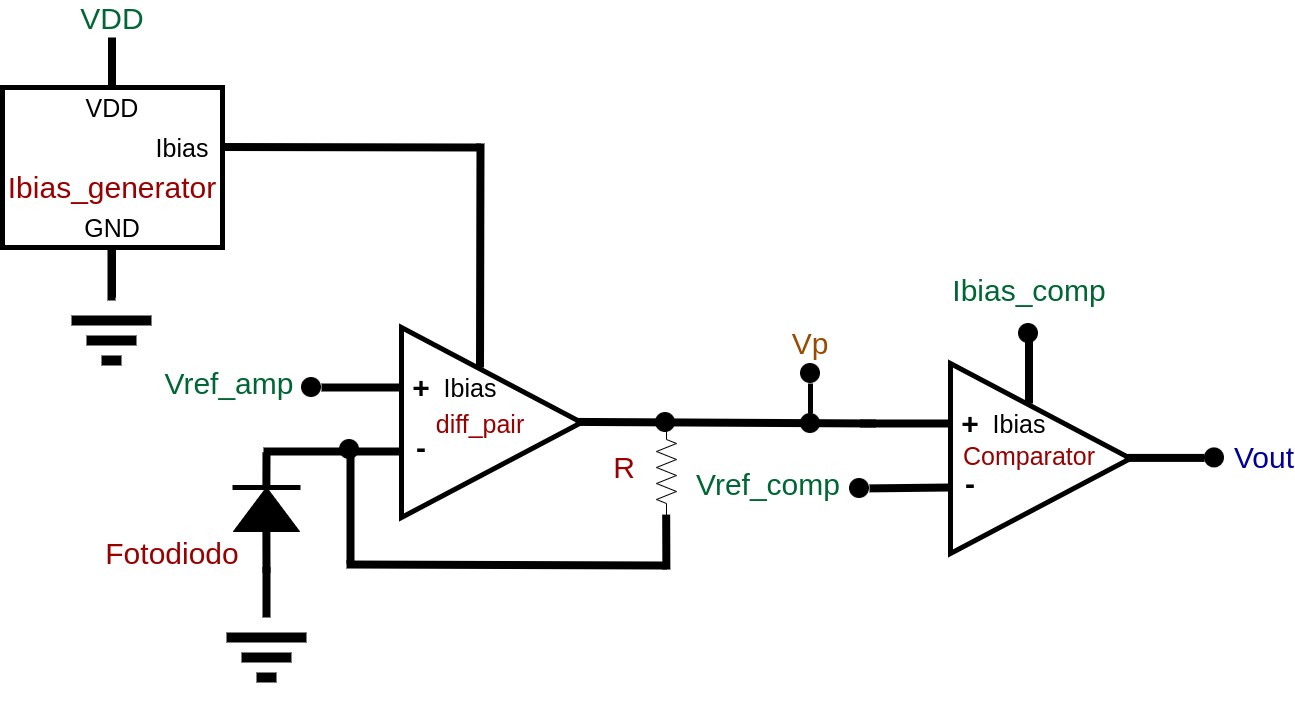
\includegraphics[scale=0.35]{Circuitos/APS_clk.png}
    \legend{Fonte: Produzido pelo autor}
\end{figure}

\begin{figure}[htb]
 \centering
    \centering
    \caption{Representa{\c c}\~ao em bloco do \NomeBloco} \label{\NomeSFig}
    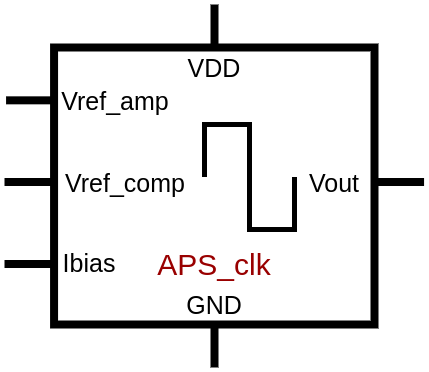
\includegraphics[scale=0.5]{Circuitos/APS_clk_block.png}
    \legend{Fonte: Produzido pelo autor}
\end{figure}

O circuito tem funcionamento similar ao do apresentado no bloco \emph{APS\_digitalized}, por\'em com apenas a sa\'ida digital sendo considerada e sendo utilizado um $TIA$ ao inv\'es de um APS. A corrente de polariza{\c c}\~ao do par diferencial \'e gerada pelo bloco Ibias\_generator presente no bloco.

Uma resist\^encia $R$ de ganho \'e utilizada, com valor apresentado na \autoref{\NomeQTab}.

\begin{table}[htb]
\caption{Resistores do bloco \NomeBloco}
\label{\NomeQTab}
\centering
\begin{tabular}{cccc}
\toprule
Resistor & W ($\mu$m)  & L ($\mu$m) & Resist\^encia (k$\Omega$)\\
\midrule \midrule
R & 1,68 & 39486,3 & 25000\\
\bottomrule
\end{tabular}
\legend{Fonte: Produzido pelo autor}
\end{table}

Para o bloco, a \autoref{eq_TIAblock} descreve $V_{PH}$, que \'e comparada com \emph{Vref\_comp} e ent\~ao utilizada para gerar o sinal de sa\'ida.

\begin{equation}
    \label{eq_TIAblock}
    V_{PH} = RI_{PH} + Vref_amp
\end{equation}

Onde:

\begin{itemize}

    \item \emph{$V_{PH}$} \'e a tens\~ao no ramo positivo do comparador [$V$]
    \item \emph{$I_{PH}$} \'e a corrente fotogerada [$A$]
    
\end{itemize}

Dois transistores NMOS n\~ao apresentados na ilustra{\c c}\~ao foram conectado com o dreno e fonte ligados ao terra e o gate em VDD, de forma a se formar um capacitor de desacoplamento para o bloco. Os par\^ametros desses transistores s\~ao dadas na \autoref{tab_capdecclk}.

\begin{table}[htbp]
\caption{Capacitores de desacoplamento via transistor do bloco \NomeBloco}
\label{tab_capdecclk}
\centering
\begin{tabular}{cccc}
\toprule
W ($\mu$m)  & L ($\mu$m) & M (n° dispositivos) & S (n° dispositivos)\\
\midrule \midrule
50 & 10 & 1 & 1\\
\bottomrule
\end{tabular}
\legend{Fonte: Produzido pelo autor}
\end{table}

Dois capacitores MOS n\~ao apresentados na ilustra{\c c}\~ao tamb\'em foram utilizados como capacitores de desacoplamento. Os par\^ametros desses capacitores s\~ao dadas na \autoref{tab_capdecclk2}.

\begin{table}[htbp]
\caption{Capacitores de desacoplamento MOS do bloco \NomeBloco}
\label{tab_capdecclk2}
\centering
\begin{tabular}{ccc}
\toprule
W ($\mu$m)  & L ($\mu$m) & Capacit\^ancia ($pF$)\\
\midrule \midrule
30 & 30 & 1,7919\\
\bottomrule
\end{tabular}
\legend{Fonte: Produzido pelo autor}
\end{table}

Dois diodos quadrados ligados reversamente em VDD e GND tamb\'em foi utilizado, com o intuito de proteger o circuito de tens\~oes reversas. Os par\^ametros desses diodos s\~ao dadas na \autoref{tab_capdecclk3}

\begin{table}[htbp]
\caption{Diodos de prote{\c c}\~ao do bloco \NomeBloco}
\label{tab_capdecclk3}
\centering
\begin{tabular}{ccc}
\toprule
W ($\mu$m)  & L ($\mu$m) & \'Area ($um^2$)\\
\midrule \midrule
3 & 3 & 9\\
\bottomrule
\end{tabular}
\legend{Fonte: Produzido pelo autor}
\end{table}
\clearpage
\renewcommand{\NomeBloco}{\textit{vref\_generator}}
\renewcommand{\NomeBlocoNoUnderline}{vrefgenerator}
\renewcommand{\NomePTab}{tab_\NomeBlocoNoUnderline}
\renewcommand{\NomeSTab}{tab_\NomeBlocoNoUnderline2}
\renewcommand{\NomePFig}{fig_\NomeBlocoNoUnderline}
\renewcommand{\NomeSFig}{fig_\NomeBlocoNoUnderline2}
\renewcommand{\NomeTTab}{tab_\NomeBlocoNoUnderline3}
\renewcommand{\NomeQTab}{tab_\NomeBlocoNoUnderline4}

\section{vref\_generator}

O \textit{\NomeBloco}\footnote{Circuito esquemático desenvolvido por \textit{Dalton Martini Colombo}} \'e o bloco respons\'avel por gerar todas as tensões de refer\^encia utilizados nos outros circuitos. O bloco apresenta as definições de sinais de entrada e sa\'ida referidos na \autoref{\NomeSTab}.

\begin{table}[htbp]
\caption{Sinais do bloco \NomeBloco}
\label{\NomeSTab}
\centering
\begin{tabular}{ccl}

    \toprule
    Sinal & Tipo    & Descrição      \\
    \midrule \midrule
    Ibias   & Entrada   & Corrente de polarização do bloco Par Diferencial \\
    \midrule
    V\_extra   & Saída   & Tensão de refer\^encia 1 \\
    \midrule
    Vref\_plus   & Saída   & Tensão de refer\^encia 2 \\
    \midrule
    Vref   & Saída   & Tensão de refer\^encia 3 \\
    \midrule
    y1   & Saída   & Tensão de refer\^encia 4 \\
    \midrule
    y2   & Saída   & Tensão de refer\^encia 5 \\
    \midrule
    y3   & Saída   & Tensão de refer\^encia 6 \\
    \midrule
    y4  & Saída   & Tensão de refer\^encia 7 \\
    \midrule
    y5   & Saída   & Tensão de refer\^encia 8 \\
    \midrule
    y6   & Saída   & Tensão de refer\^encia 9 \\
    \bottomrule
\end{tabular}
\legend{Fonte: Produzido pelo autor}
\end{table}

O circuito projetado para o bloco \'e demonstrado na \autoref{\NomePFig}.

\begin{figure}[htb]
 \label{\NomePFig}
 \centering
    \centering
    \caption{Circuito CMOS projetado para o bloco \NomeBloco} 
    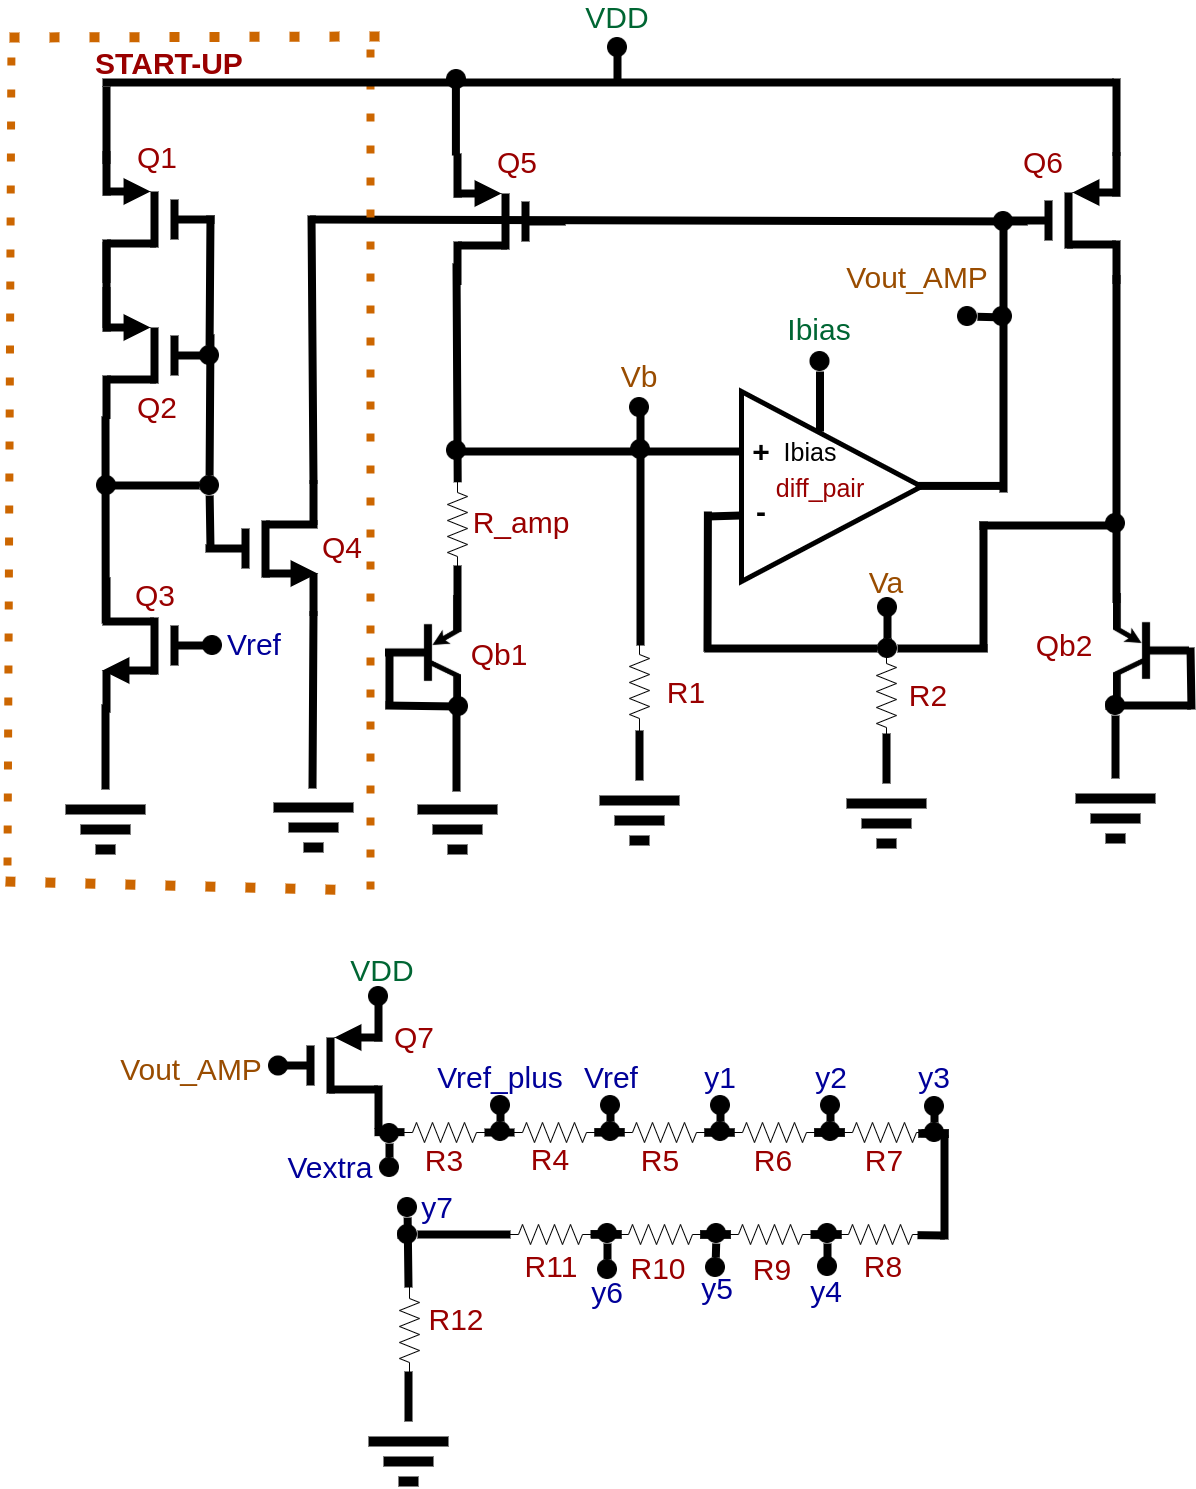
\includegraphics[scale=0.3]{Circuitos/vref_generator.png}
    \legend{Fonte: Produzido pelo autor}
\end{figure}

\begin{figure}[htb]
 \centering
    \centering
    \caption{Representação em bloco do \NomeBloco} \label{\NomeSFig}
    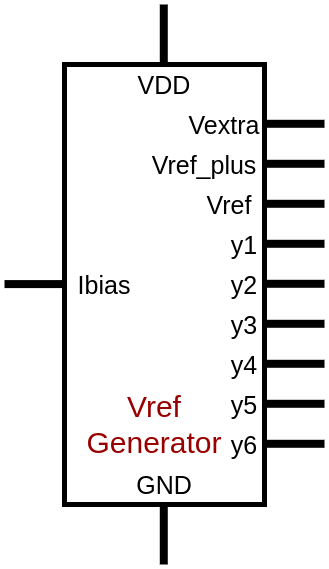
\includegraphics[scale=0.3]{Circuitos/vref_generator_block.png}
    \legend{Fonte: Produzido pelo autor}
\end{figure}

Os transistores utilizados no bloco \NomeBloco{} apresentam os par\^ametros mostrados na \autoref{\NomeTTab}.

\begin{table}[htbp]
\caption{Transistores do Bloco \NomeBloco}
\label{\NomeTTab}
\centering
\begin{tabular}{ccccc}
\toprule
Transistor & W ($\mu$m)  & L ($\mu$m)           & M (n° dispositivos) & S (n° dispositivos)\\
\midrule \midrule
Q1 e Q2 & 0,5 & 19,995 & 1 & 1\\
\midrule
Q3 & 20 & 0,18 & 1 & 1\\
\midrule
Q4 & 2 & 0,18 & 1 & 1\\
\midrule
Q5, Q6 e Q7 & 20 & 16 & 4 & 1\\
\midrule
Qb1 (PNP) & 5 & 5 & 1 & 1\\
\midrule
Qb2 (PNP) & 5 & 5 & 8 & 1\\
\bottomrule
\end{tabular}
\legend{Fonte: Produzido pelo autor}
\end{table}

Os resistores utilizados no bloco \NomeBloco{} apresentam os par\^ametros mostrados na \autoref{\NomeQTab}.

\begin{table}[htbp]
\caption{Resistores do bloco \NomeBloco}
\label{\NomeQTab}
\centering
\begin{tabular}{cccccc}
\toprule
Resistor & \begin{tabular}[c]{@{}c@{}}W \\($\mu$m)\end{tabular}   & \begin{tabular}[c]{@{}c@{}}L \\($\mu$m)\end{tabular}  & \begin{tabular}[c]{@{}c@{}}Resist\^encia\\ (k$\Omega$)\end{tabular} & \begin{tabular}[c]{@{}c@{}}M\\(n° dispositivos)\end{tabular} & \begin{tabular}[c]{@{}c@{}}S \\(n° dispositivos)\end{tabular}\\
\midrule \midrule
R1 e R2 & 2 & 18,85 & 10,1024 & 1 & 10\\
\midrule
\begin{tabular}[c]{@{}c@{}}R\_amp, R3, R4,\\ R5, R6, R7, \\ R8, R9, R10, \\ R11\end{tabular} & 2 & 18,85 & 10,1024 & 1 & 1\\
\midrule
R12 & 2 & 18,85 & 10,1024 & 7 & 1\\
\bottomrule
\end{tabular}
\legend{Fonte: Produzido pelo autor}
\end{table}

O dispositivo funciona produzindo uma corrente de refer\^encia extremamente est\'avel, utilizando um amplificador operacional e realimentação. O braço \textit{Q7} utiliza dessa corrente como refer\^encia para gerar uma corrente que alimenta alguns resistores, que geram os potenciais de refer\^encia desejados.

\renewcommand{\NomeBloco}{\emph{vref\_block}}
\newcommand{\NomeBlocoA}{vrefblock}
\renewcommand{\NomePTab}{tab_\NomeBlocoA}
\renewcommand{\NomeSTab}{tab_\NomeBlocoA2}
\renewcommand{\NomePFig}{fig_\NomeBlocoA}
\renewcommand{\NomeSFig}{fig_\NomeBlocoA2}
\renewcommand{\NomeTTab}{tab_\NomeBlocoA3}

\section{vref\_block}

O bloco \NomeBloco{} tem a finalidade de conter o bloco \emph{vref\_generator}, mais o bloco respons\'avel por gerar a corrente que o polariza. O bloco apresenta as definições de sinais de entrada e sa\'ida referidos na \autoref{\NomeSTab}.

\begin{table}[!h] 
\caption{Sinais do bloco \NomeBloco}
\label{\NomeSTab}
\centering
\begin{tabular}{ccl}

    \toprule
    Sinal & Tipo    & Descrição      \\
    \midrule \midrule
    V\_extra   & Saída   & Tensão de refer\^encia 1 \\
    \midrule
    Vref\_plus   & Saída   & Tensão de refer\^encia 2 \\
    \midrule
    Vref   & Saída   & Tensão de refer\^encia 3 \\
    \midrule
    Vref\_minus   & Saída   & Tensão de refer\^encia 4 \\
    \midrule
    Vref\_minus2   & Saída   & Tensão de refer\^encia 5 \\
    \midrule
    Vref\_minus3   & Saída   & Tensão de refer\^encia 6 \\
    \midrule
    Vref\_minus4  & Saída   & Tensão de refer\^encia 7 \\
    \midrule
    Vref\_minus5   & Saída   & Tensão de refer\^encia 8 \\
    \midrule
    Vref\_minus6   & Saída   & Tensão de refer\^encia 9 \\
    \bottomrule
\end{tabular}
\legend{Fonte: Produzido pelo autor}
\end{table}

O circuito projetado para o bloco \'e demonstrado na \autoref{\NomePFig}.

\begin{figure}[htb]
 \centering
    \centering
    \caption{\label{\NomePFig}Circuito CMOS projetado para o bloco \NomeBloco}
    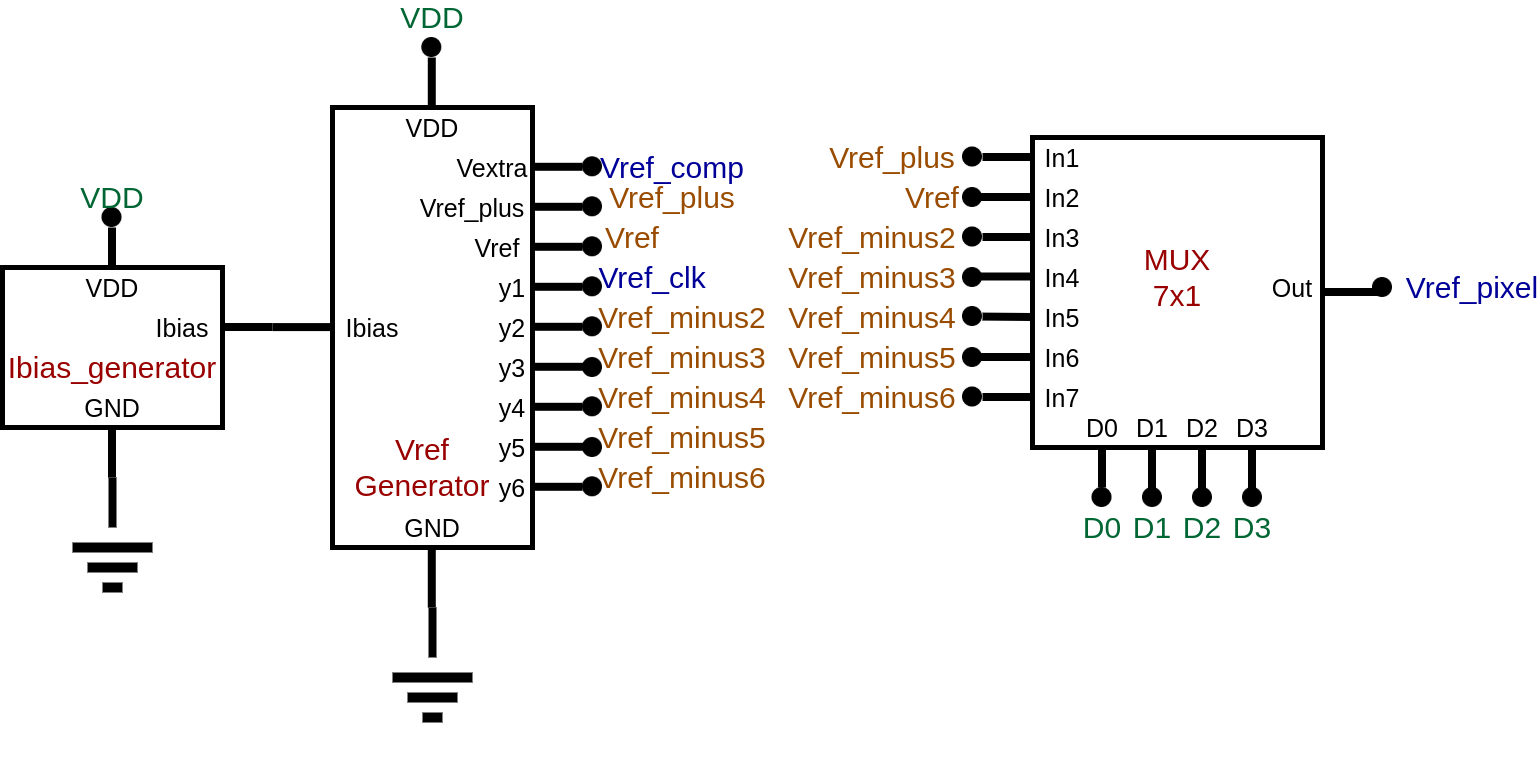
\includegraphics[scale=0.3]{Circuitos/vref_block.png}
    \legend{Fonte: Produzido pelo autor}
\end{figure}

\begin{figure}[htb]
 \centering
    \centering
    \caption{\label{\NomeSFig}Representação em bloco do \NomeBloco}
    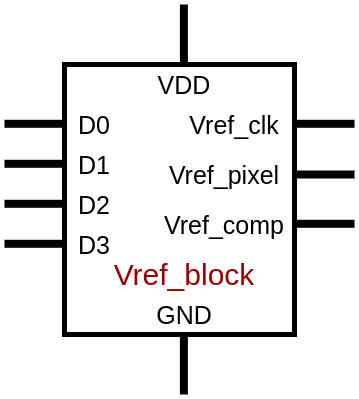
\includegraphics[scale=0.3]{Circuitos/vref_block_block.png}
    \legend{Fonte: Produzido pelo autor}
\end{figure}

\renewcommand{\NomeBloco}{\emph{vref\_block\_with\_mux}}
\renewcommand{\NomeBlocoA}{vrefblockwithmux}
\renewcommand{\NomePTab}{tab_\NomeBlocoA}
\renewcommand{\NomeSTab}{tab_\NomeBlocoA2}
\renewcommand{\NomePFig}{fig_\NomeBlocoA}
\renewcommand{\NomeSFig}{fig_\NomeBlocoA2}
\renewcommand{\NomeTTab}{tab_\NomeBlocoA3}

\section{\NomeBloco}

O bloco \NomeBloco{} tem a finalidade de selecionar a tens\~ao de refer\^encia a ser utilizada nos blocos de compara{\c c}\~ao do circuito, al\'em de retornar a tens\~ao de refer\^encia utilizada pelo bloco \emph{TIA}. A \autoref{\NomePTab} indica a Tabela Verdade do bloco. Embora tenha uma l\'ogica digital, o circuito permite sa\'idas anal\'ogicas.

\begin{table}[htbp]

\caption{Tabela Verdade do bloco \NomeBloco}%
\label{\NomePTab}
\centering
\begin{tabular}{ccccc}
    \toprule
    D0 & D1 & D2 & D3 & Out \\
    \midrule \midrule
    0 & 0 & 0 & 0 & Vref\_plus\\
    \midrule
    0 & 1 & 0 & 0 & Vref\\
    \midrule
    1 & 0 & 0 & 0 & Vref\_minus2\\
    \midrule
    1 & 1 & 0 & 0 & Vref\_minus3\\
    \midrule
    X & X & 0 & 1 & Vref\_minus4\\
    \midrule
    X & X & 1 & 0 & Vref\_minus5\\
    \midrule
    X & X & 1 & 1 & Vref\_minus6\\
\bottomrule

\end{tabular}
\fonte{Produzido pelo autor.}
\end{table}

O bloco apresenta as defini{\c c}\~oes de sinais de entrada e sa\'ida referidos na \autoref{\NomeSTab}.

\begin{table}[htbp]
\caption{Sinais do bloco \NomeBloco}
\label{\NomeSTab}
\centering
\begin{tabular}{ccl}

    \toprule
    Sinal & Tipo    & Descri{\c c}\~ao      \\
    \midrule \midrule
    D0   & Entrada   & Entrada de sele{\c c}\~ao 1 \\
    \midrule
    D1   & Entrada   & Entrada de sele{\c c}\~ao 2 \\
    \midrule
    D2   & Entrada   & Entrada de sele{\c c}\~ao 3 \\
    \midrule
    D3   & Entrada   & Entrada de sele{\c c}\~ao 4 \\
    \midrule
    Vref\_pixel   & Sa\'ida   & Tens\~ao de refer\^encia selecionada \\
    \midrule
    Vref\_clk¹  & Sa\'ida   & Tens\~ao de refer\^encia do Clock \\
    \midrule
    Vref\_comp²  & Sa\'ida   & Tens\~ao de refer\^encia do Clock do bloco teste \\
    \bottomrule
\end{tabular}
\legend{Fonte: Produzido pelo autor}
\legend{¹ Essa tens\~ao \'e igual \'a sa\'ida Vref\_minus do bloco \emph{vref\_block}\\² Essa tens\~ao \'e igual \'a sa\'ida Vref\_extra do bloco \emph{vref\_block}}
\end{table}

O circuito projetado para o bloco \'e demonstrado na \autoref{\NomePFig}.

\begin{figure}[htb]
 \label{NomePFig}
 \centering
    \centering
    \caption{Circuito CMOS projetado para o bloco \NomeBloco} \label{\NomePFig}
    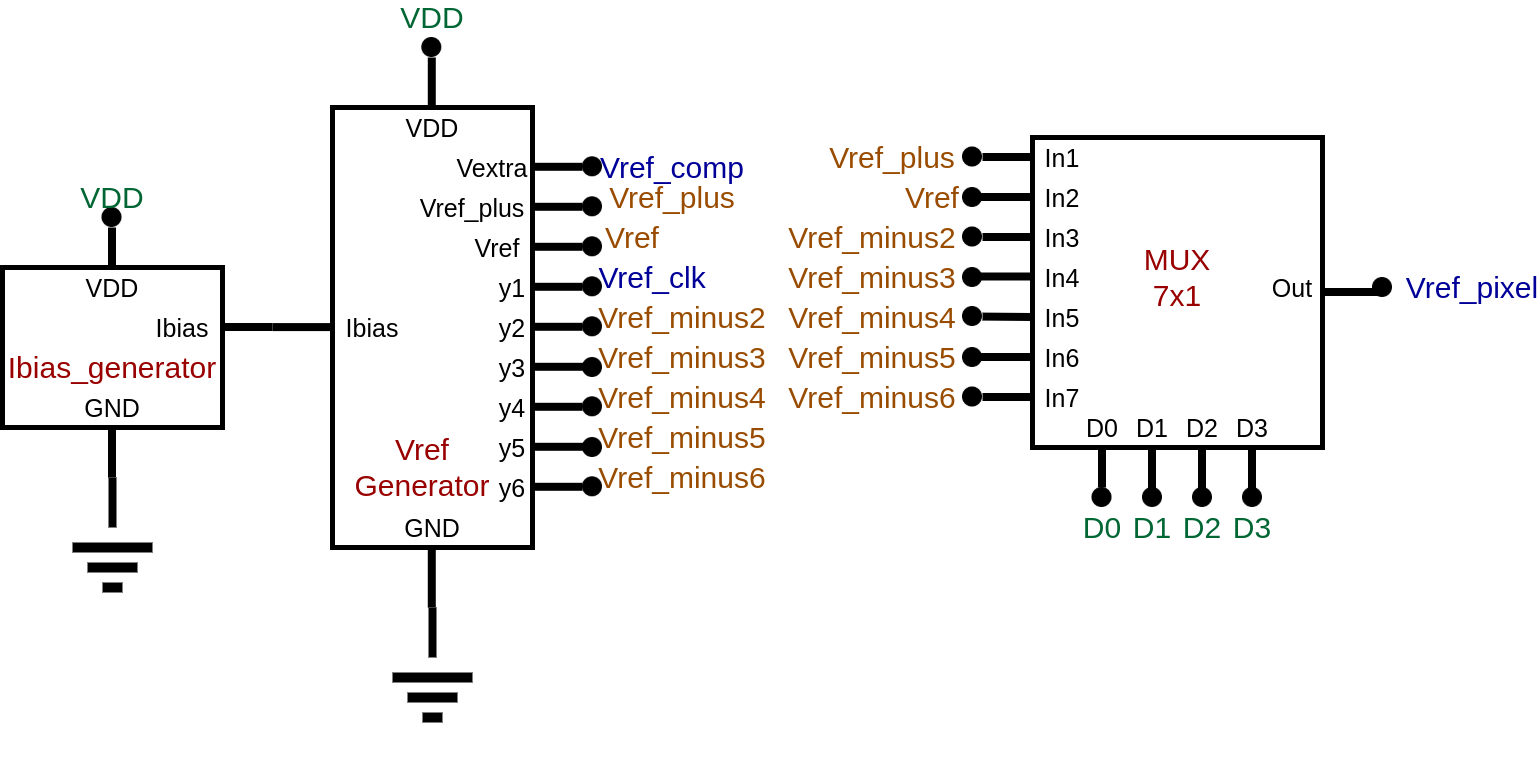
\includegraphics[scale=0.28]{Circuitos/vref_block.png}
    \legend{Fonte: Produzido pelo autor}
\end{figure}

\begin{figure}[htb]
 \label{NomeSFig}
 \centering
    \centering
    \caption{Representa{\c c}\~ao em bloco do \NomeBloco} \label{NomeSFig}
    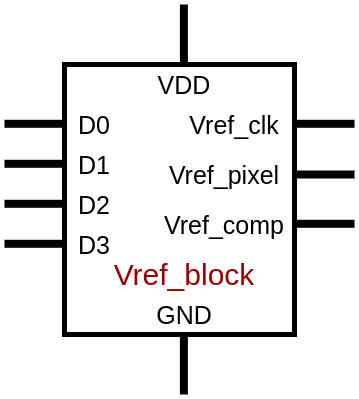
\includegraphics[scale=0.3]{Circuitos/vref_block_block.png}
    \legend{Fonte: Produzido pelo autor}
\end{figure}

\renewcommand{\NomeBloco}{ibias\_block}
\renewcommand{\NomeBlocoA}{ibiasblock}
\renewcommand{\NomePTab}{tab_\NomeBlocoA}
\renewcommand{\NomeSTab}{tab_\NomeBlocoA2}
\renewcommand{\NomePFig}{fig_\NomeBlocoA}
\renewcommand{\NomeSFig}{fig_\NomeBlocoA2}
\renewcommand{\NomeTTab}{tab_\NomeBlocoA3}

O bloco \NomeBloco{} gera diversos drenos de corrente utilizadas por outros blocos. O bloco apresenta as defini{\c c}\~oes de sinais de entrada e sa\'ida referidos na \autoref{\NomeSTab}.

\begin{table}[htbp]
\caption{Sinais do bloco \NomeBloco}
\label{\NomeSTab}
\centering
\begin{tabular}{ccl}

    \toprule
    Sinal & Tipo    & Descri{\c c}\~ao      \\
    \midrule \midrule
    bias\_pixel\_1   & Sa\'ida   & Dreno de corrente para o APS 1 (0,5 $\mu$A) \\
    \midrule
    bias\_pixel\_2   & Sa\'ida   & Dreno de corrente para o APS 2 (0,5 $\mu$A) \\
    \midrule
    bias\_pixel\_3   & Sa\'ida   & Dreno de corrente para o APS 3 (0,5 $\mu$A) \\
    \midrule
    bias\_pixel\_4   & Sa\'ida   & Dreno de corrente para o APS 4 (0,5 $\mu$A) \ \\
    extra\_500nA   & Sa\'ida   & Dreno de corrente para o APS de teste (0,5 $\mu$A) \ \\
    \midrule
    bias\_comp\_1   & Sa\'ida   & Dreno de corrente para o Comparador 1 (1,5 $\mu$A) \ \\
    \midrule
    bias\_comp\_2   & Sa\'ida   & Dreno de corrente para o Comparador 2 (1,5 $\mu$A) \ \\
    \midrule
    bias\_comp\_3   & Sa\'ida   & Dreno de corrente para o Comparador 3 (1,5 $\mu$A) \\
    \midrule
    bias\_comp\_4   & Sa\'ida   & Dreno de corrente para o Comparador 4 (1,5 $\mu$A) \\
    extra\_1500nA   & Sa\'ida   & Dreno de corrente para o Comparador de teste (1,5 $\mu$A) \ \\
    \bottomrule
\end{tabular}
\legend{Fonte: Produzido pelo autor}
\legend{¹ Essa tens\~ao \'e igual \'a sa\'ida Vref\_minus do bloco \emph{vref\_block}\\² Essa tens\~ao \'e igual \'a sa\'ida Vref\_extra do bloco \emph{vref\_block}}
\end{table}

O circuito projetado para o bloco \'e demonstrado na \autoref{\NomePFig}.

\begin{figure}[htb]
 \label{NomePFig}
 \centering
    \centering
    \caption{Circuito CMOS projetado para o bloco \NomeBloco} \label{\NomePFig}
    \includegraphics[scale=0.38]{Circuitos/ibias_block.png}
    \legend{Fonte: Produzido pelo autor}
\end{figure}

\begin{figure}[htb]
 \label{NomeSFig}
 \centering
    \centering
    \caption{Representa{\c c}\~ao em bloco do \NomeBloco} \label{NomeSFig}
    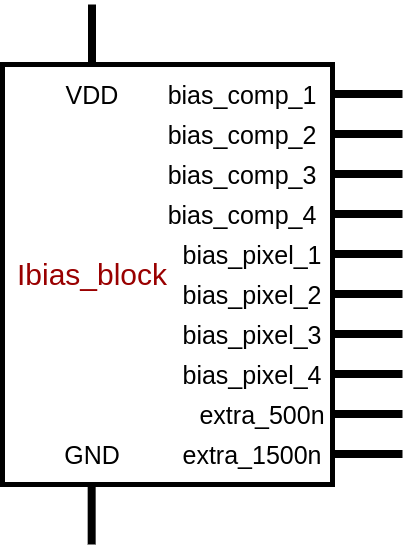
\includegraphics[scale=0.3]{Circuitos/ibias_block_block.png}
    \legend{Fonte: Produzido pelo autor}
\end{figure}
\clearpage
\renewcommand{\NomeBloco}{\textit{APS\_3}}
\renewcommand{\NomeBlocoNoUnderline}{apsthree}
\renewcommand{\NomePTab}{tab_\NomeBlocoNoUnderline}
\renewcommand{\NomeSTab}{tab_\NomeBlocoNoUnderline2}
\renewcommand{\NomePFig}{fig_\NomeBlocoNoUnderline}
\renewcommand{\NomeSFig}{fig_\NomeBlocoNoUnderline2}
\renewcommand{\NomeTTab}{tab_\NomeBlocoNoUnderline3}
\renewcommand{\NomeQTab}{tab_\NomeBlocoNoUnderline4}

\section{APS\_3}

O \textit{\NomeBloco} \'e o circuito respons\'avel por armazenar todos os tr\^es blocos APS de cor (Azul, Verde, Vermelho), mais o TIA geradora de rel\'ogio de refer\^encia para os APS's citados. O bloco apresenta as definicões de sa\'ida referidos na \autoref{\NomeSTab}.

\begin{figure}[!h]
 \centering
    \centering
    \caption{\label{\NomeSFig}Representacão em bloco do \NomeBloco}
    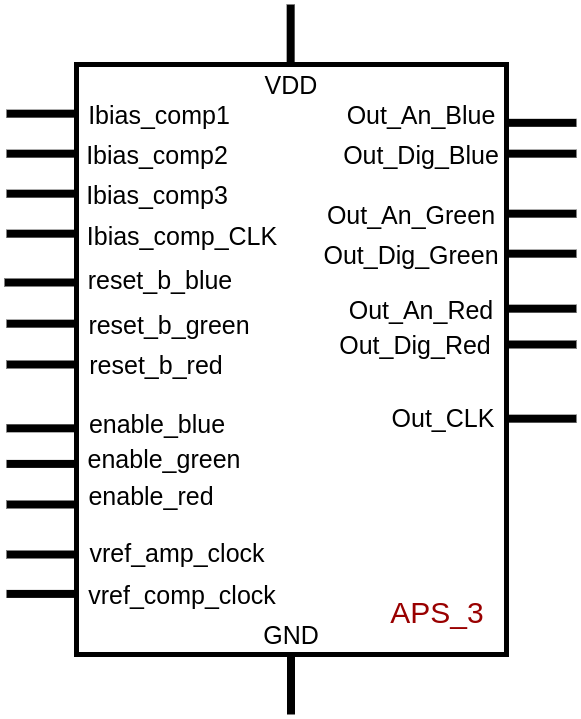
\includegraphics[scale=0.3]{Circuitos/APS_3_block.png}
    \legend{Fonte: Produzido pelo autor}
\end{figure}

\begin{table}[!h]
\centering
  \caption{Descricão dos sinais de entrada e sa\'ida do circuito projetado para as cores azul, verde e vermelha}%
  \label{\NomeSTab}
  \begin{tabular}{ccll}
  \toprule
   Sinal & Tipo & Descricão & Observacão \\
  \midrule \midrule
   RESET\_BLUE & Entrada & \begin{tabular}[l]{@{}l@{}}Sinal de tensão \textit{RESET}\\ no APS para cor azul\end{tabular} & Ativo em n\'ivel baixo \\
  \midrule
   RESET\_GREEN & Entrada & \begin{tabular}[l]{@{}l@{}}Sinal de tensão de \textit{RESET}\\ no APS para cor verde\end{tabular} & Ativo em n\'ivel baixo \\
  \midrule
   RESET\_RED & Entrada & \begin{tabular}[l]{@{}l@{}}Sinal de tensão \textit{RESET}\\ no APS para cor vermelha\end{tabular} & Ativo em n\'ivel baixo \\
   \midrule
   ENABLE\_BLUE & Entrada & \begin{tabular}[l]{@{}l@{}}Sinal de tensão \textit{ENABLE} \\no APS para cor azul\end{tabular} & Ativo em n\'ivel alto \\
  \midrule
   ENABLE\_GREEN & Entrada & \begin{tabular}[l]{@{}l@{}}Sinal de tensão \textit{ENABLE} \\no APS para cor verde\end{tabular} & Ativo em n\'ivel alto \\
  \midrule
   ENABLE\_RED & Entrada & \begin{tabular}[l]{@{}l@{}}Sinal de tensão \textit{ENABLE}\\ no APS para cor vermelha\end{tabular} & Ativo em n\'ivel alto \\
  \midrule
   Ibias\_comp1 & Entrada & \begin{tabular}[l]{@{}l@{}}Fonte de corrente para\\ cor Azul\end{tabular} &  \\
   \midrule
   Ibias\_comp2 & Entrada & \begin{tabular}[l]{@{}l@{}}Fonte de corrente para\\ cor Verde\end{tabular} &  \\
   \midrule
   Ibias\_comp3 & Entrada & \begin{tabular}[l]{@{}l@{}}Fonte de corrente para\\ cor Vermelha\end{tabular} &  \\
   \midrule
   Ibias\_clk & Entrada & \begin{tabular}[l]{@{}l@{}}Fonte de corrente para o\\ bloco \textit{APS\_pixel\_clk}\end{tabular}
    &  \\
  \midrule
   Out\_An\_Blue & Sa\'ida & \begin{tabular}[l]{@{}l@{}}Sinal anal\'ogico para cor\\ azul\end{tabular} \\
  \midrule
   Out\_Dig\_Blue & Sa\'ida & Sinal digital para cor azul \\
  \midrule
   Out\_An\_Green & Sa\'ida & \begin{tabular}[l]{@{}l@{}}Sinal anal\'ogico para cor\\ verde\end{tabular} \\
  \midrule
   Out\_Dig\_Green & Sa\'ida & Sinal digital para cor verde \\
  \midrule
   Out\_An\_Red & Sa\'ida & \begin{tabular}[l]{@{}l@{}}Sinal anal\'ogico para cor\\ vermelha\end{tabular} \\
  \midrule
   Out\_Dig\_Red & Sa\'ida & \begin{tabular}[l]{@{}l@{}}Sinal digital para cor\\ vermelha\end{tabular} \\
  \bottomrule
  \end{tabular}
  \legend{Fonte: Produzido pelo autor.}
\end{table}

O circuito projetado para o bloco \'e demonstrado na \autoref{\NomePFig}.

\clearpage

\begin{figure}[!h]
 \centering
    \centering
    \caption{Circuito CMOS projetado para o bloco \NomeBloco} 
    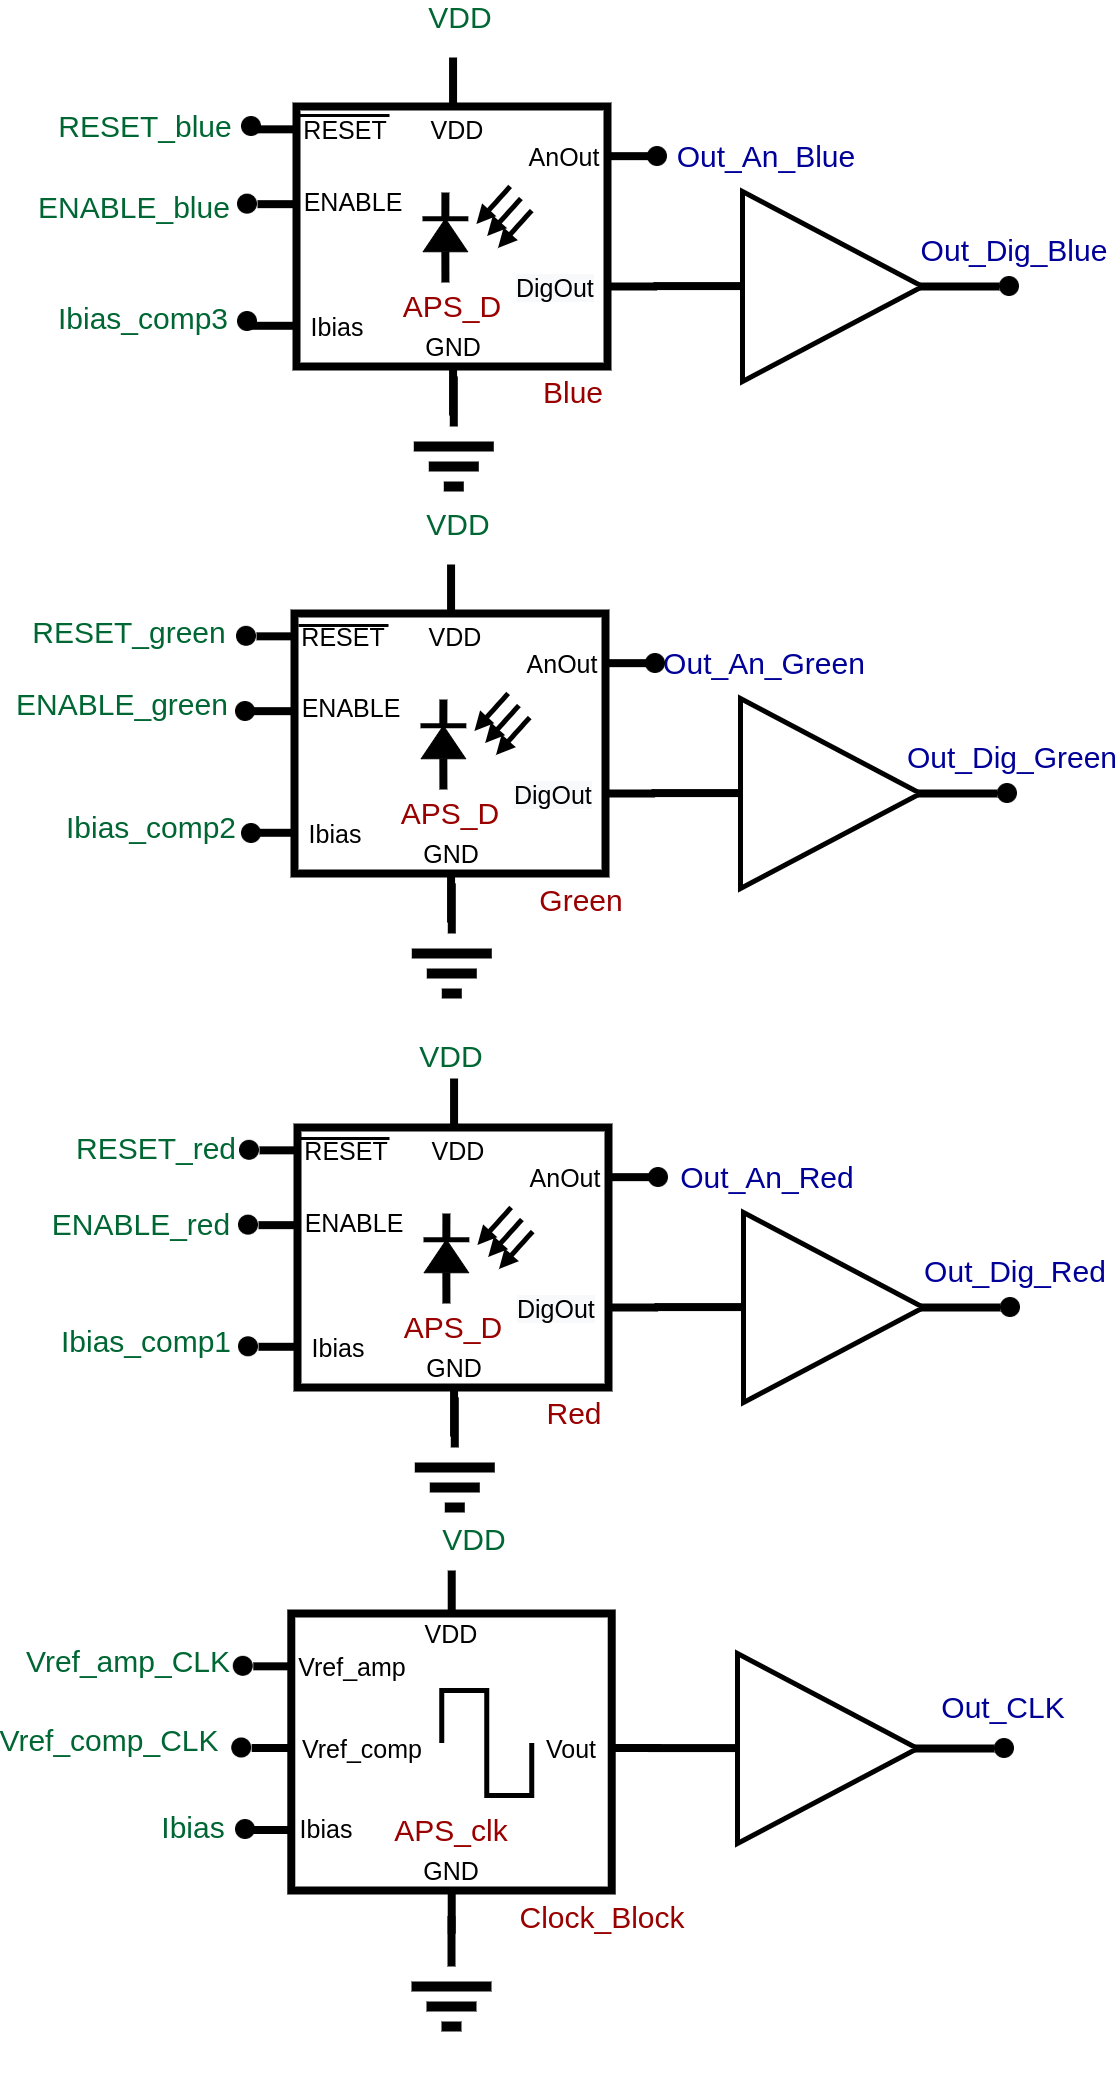
\includegraphics[scale=0.3]{Circuitos/APS_3.png}
    \legend{Fonte: Produzido pelo autor}
    \label{\NomePFig}
\end{figure}

As sa\'idas digitais de cada bloco APS\_digitalized apresentam um buffer, de forma a garantir a integridade do sinal nos pinos do Circuito Integrado.
\renewcommand{\NomeBloco}{\emph{Comparador}}
\renewcommand{\NomeBlocoNoIt}{Comparador}
\renewcommand{\NomePTab}{tab_\NomeBloco}
\renewcommand{\NomeSTab}{tab_\NomeBlocoNoIt2}
\renewcommand{\NomePFig}{fig_\NomeBlocoNoIt}
\renewcommand{\NomeSFig}{fig_\NomeBlocoNoIt2}
\renewcommand{\NomeTTab}{tab_\NomeBlocoNoIt3}

\section{\NomeBloco}

O bloco \NomeBloco{} tem a fun{\c c}\~ao de comparar dois sinais anal\'ogicos advindos nas entradas '+' (\emph{Vp}) e '-' (\emph{Vn}), e retornar \emph{VDD} caso Vp seja maior do que Vn, e \emph{GND} caso Vp seja menor ou igual a Vn.  O bloco apresenta as defini{\c c}\~oes de sinais de entrada e sa\'ida referidos na \autoref{\NomeSTab}.

\begin{table}[htbp]
\caption{Sinais do bloco \NomeBloco}
\label{\NomeSTab}
\centering
\begin{tabular}{ccl}

    \toprule
    Sinal & Tipo    & Descri{\c c}\~ao        \\
    \midrule \midrule
    Vp (+) & Entrada & Entrada positiva do Comparador\\
    \midrule
    Vn (-) & Entrada & Entrada negativa do Comparador\\
    \midrule
    Ibias & Entrada & Corrente de polariza{\c c}\~ao do Comparador\\
    \midrule
    Vo & sa\'ida & Sa\'ida do Comparador\\
    \bottomrule
\end{tabular}
\legend{Fonte: Produzido pelo autor}
\end{table}

O circuito projetado para o bloco \'e demonstrado na \autoref{\NomePFig}.

\begin{figure}[htb]
 \label{\NomePFig}
 \centering
    \centering
    \caption{Circuito CMOS projetado para o bloco \NomeBloco} 
    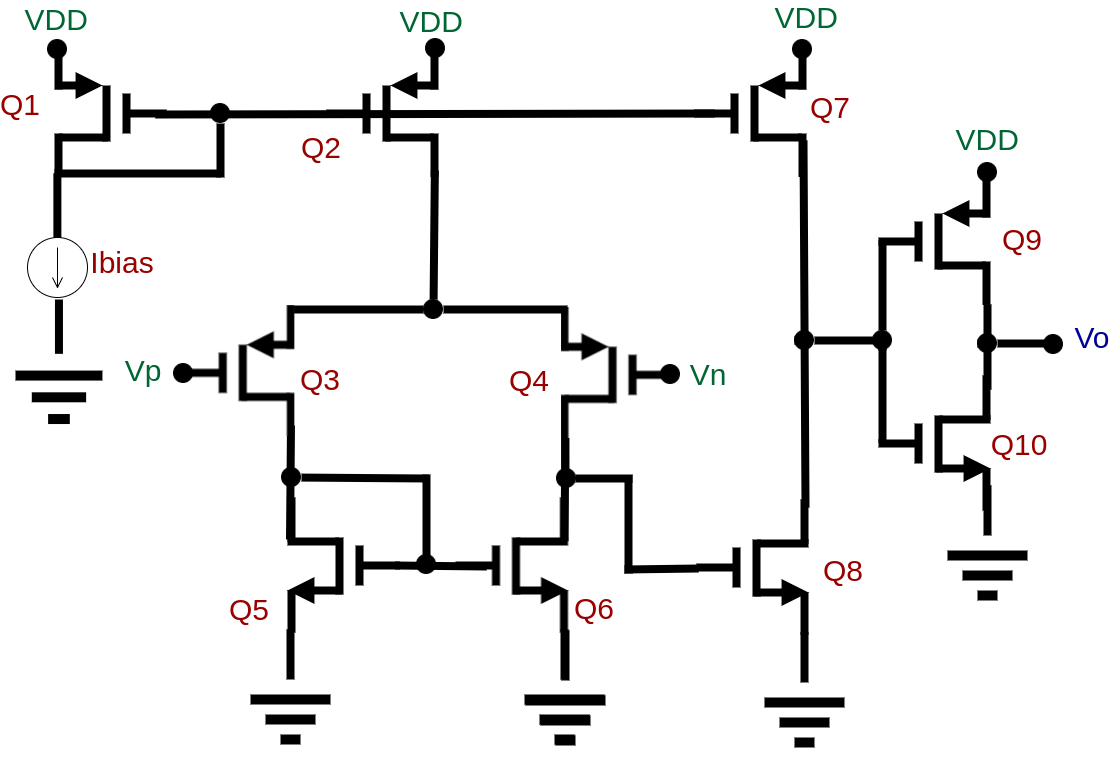
\includegraphics[scale=0.3]{Circuitos/Comparator.png}
    \legend{Fonte: Produzido pelo autor}
\end{figure}

\begin{figure}[htb]
 \centering
    \centering
    \caption{Representa{\c c}\~ao em bloco do \NomeBloco} \label{\NomeSFig}
    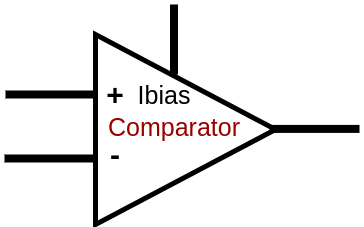
\includegraphics[scale=0.3]{Circuitos/Comparator_block.png}
    \legend{Fonte: Produzido pelo autor}
\end{figure}

Os transistores utilizados no bloco \NomeBloco{} apresentam os par\^ametros mostrados na \autoref{\NomeTTab}.

\begin{table}[htbp]
\caption{Transistores do Bloco \NomeBloco}
\label{\NomeTTab}
\centering
\begin{tabular}{ccccc}
\toprule
Transistor & W ($\mu$m)  & L ($\mu$m)           & M (n° dispositivos) & S (n° dispositivos)\\
\midrule \midrule
Q1 & 10 & 1 & 1 & 1\\
\midrule
Q2$^1$ & 10 & 1 & 6 & 6\\
\midrule
Q3 & 4 & 1 & 2 & 2\\
\midrule
Q4 & 4 & 1 & 2 & 2\\
\midrule
Q5 & 2 & 1 & 2 & 2\\
\midrule
Q6 & 2 & 1 & 2 & 2\\
\midrule
Q7$^1$ & 10 & 1 & 8 & 8\\
\midrule
Q8 & 2 & 1 & 4 & 4\\
\midrule
Q9 & 3 & 0.18 & 1 & 1\\
\midrule
Q10 & 1.5 & 0.18 & 1 & 1\\

\bottomrule
\end{tabular}
\legend{Fonte: Produzido pelo autor}
\legend{$^1$Calculado de forma a produzir uma corrente de 9 $\mu$A}
\end{table}
 
O \NomeBloco{} \'e desenvolvido com tr\^es est\'agios de amplifica{\c c}\~ao. O primeiro est\'agio, composto pelos transistores Q3, Q4, Q5, Q6 t\^em a fun{\c c}\~a de realizar a diferen{\c c}a entra as entradas \emph{Vp} e \emph{Vn} e multiplicar por um pequeno ganho. Os transistores Q3 e Q4 sao respons\'aveis por receber as entradas, enquanto os transistores Q5 e Q6 funcionam como transistores de Carga Ativa. O Q2 funciona como uma fonte de corrente.

O segundo est\'agio \'e um est\'agio de ganho, do qual o transistor Q2 fornece um ganho para a saida do est\'agio anterior e o transistor Q7 funciona como uma fonte de corrente para o est\'agio.

Diodos quadrados \emph{D1} e \emph{D2} de prote{\c c}\~ao s\~ao inclu\'idos nos terminais \emph{Vp} e \emph{Vn do circuito}, com \^anodo ligado ao terra e catodo ligado ao seu respectivo terminal. Os diodo apresentam os seguintes par\^ametros apresentados na \autoref{diodosComp}.

\begin{table}[htbp]
\caption{Diodos do Bloco \NomeBloco}
\label{diodosComp}
\centering
\begin{tabular}{cccc}
\toprule
Diodo & W ($\mu$m)  & L ($\mu$m)           & \'Area ($\mu$m²)\\
\midrule \midrule
D1 e D2 & 1 & 1 & 1 \\

\bottomrule
\end{tabular}
\legend{Fonte: Produzido pelo autor}
\end{table}

\section{Circuitos de Teste}
\label{BlocoTestes}

O circuito apresenta dois circuitos de teste adicionais, sendo um para um APS e outro para o TIA. A finalidade destes circuitos \'e de testar o sistema sem a necessidade de uma fonte luminosa. Para isso \'e acrescentado um pino diretamente aos catodos dos fotodiodos, em que uma tensão pode ser diretamente injetada nos mesmos de forma a simular a fotogeração.

O APS de teste utiliza os pinos de RESET e ENABLE iguais ao do APS de cor azul, mas \'e polarizado com uma fonte de corrente pr\'opria e também apresenda sa\'idas pr\'oprias. Caso se mantenha o pino de injeção de corrente flutuante, o APS deve funcionar de forma equivalente aos outros.